\documentclass[a4paper]{article}
\usepackage{vntex}
%\usepackage[english,vietnam]{babel}
%\usepackage[utf8]{inputenc}

%\usepackage[utf8]{inputenc}
%\usepackage[francais]{babel}
\usepackage{a4wide,amssymb,epsfig,latexsym,array,hhline,fancyhdr}

\usepackage{amsmath}
\usepackage{amsthm}
\usepackage{multicol,longtable,amscd}
\usepackage{diagbox}%Make diagonal lines in tables
\usepackage{booktabs}
\usepackage{alltt}
\usepackage[framemethod=tikz]{mdframed}% For highlighting paragraph backgrounds
\usepackage{caption,subcaption}
\usepackage{vhistory}
\usepackage{lastpage}
\usepackage[lined,boxed,commentsnumbered]{algorithm2e}
\usepackage{enumerate}
\usepackage{color}
\usepackage{graphicx}							% Standard graphics package
\usepackage{array}
\usepackage{tabularx, caption}
\usepackage{multirow}
\usepackage{multicol}
\usepackage{rotating}
\usepackage{graphics}
\usepackage{geometry}
\usepackage{setspace}
\usepackage{epsfig}
\usepackage{tikz}
\usetikzlibrary{arrows,snakes,backgrounds}
\usepackage[unicode]{hyperref}
\hypersetup{urlcolor=blue,linkcolor=black,citecolor=black,colorlinks=true} 
%\usepackage{pstcol} 								% PSTricks with the standard color package

\newtheorem{theorem}{{\bf Định lý}}
\newtheorem{property}{{\bf Tính chất}}
\newtheorem{proposition}{{\bf Mệnh đề}}
\newtheorem{corollary}[proposition]{{\bf Hệ quả}}
\newtheorem{lemma}[proposition]{{\bf Bổ đề}}


%\usepackage{fancyhdr}
\setlength{\headheight}{40pt}
\pagestyle{fancy}
\fancyhead{} % clear all header fields
\fancyhead[L]{
 \begin{tabular}{rl}
    \begin{picture}(25,15)(0,0)
    \put(0,-8){
\includegraphics[width=8mm, height=8mm]{Images/hcmut.png}}
    %\put(0,-8){\epsfig{width=10mm,figure=hcmut.eps}}
   \end{picture}&
	%
\includegraphics[width=8mm, height=8mm]{hcmut.png} & %
	\begin{tabular}{l}
		\textbf{\bf \ttfamily Trường Đại Học Bách Khoa Tp.Hồ Chí Minh}\\
		\textbf{\bf \ttfamily Khoa Khoa Học và Kỹ Thuật Máy Tính}
	\end{tabular} 	
 \end{tabular}
}
\fancyhead[R]{
	\begin{tabular}{l}
		\tiny \bf \\
		\tiny \bf 
	\end{tabular}  }
\fancyfoot{} % clear all footer fields
\fancyfoot[L]{\scriptsize \ttfamily Công nghệ phần mềm - Niên khóa 2021-2022}
\fancyfoot[R]{\scriptsize \ttfamily Trang {\thepage}/\pageref{LastPage}}
\renewcommand{\headrulewidth}{0.3pt}
\renewcommand{\footrulewidth}{0.3pt}


%%%
\setcounter{secnumdepth}{4}
\setcounter{tocdepth}{3}
\makeatletter
\newcounter {subsubsubsection}[subsubsection]
\renewcommand\thesubsubsubsection{\thesubsubsection .\@alph\c@subsubsubsection}
\newcommand\subsubsubsection{\@startsection{subsubsubsection}{4}{\z@}%
                                     {-3.25ex\@plus -1ex \@minus -.2ex}%
                                     {1.5ex \@plus .2ex}%
                                     {\normalfont\normalsize\bfseries}}
\newcommand*\l@subsubsubsection{\@dottedtocline{3}{10.0em}{4.1em}}
\newcommand*{\subsubsubsectionmark}[1]{}
\makeatother
%make in-line maths symbols blue to read/check easily

\sloppy
\captionsetup[figure]{labelfont={small,bf},textfont={small,it},belowskip=-1pt,aboveskip=-9pt}
%space remove between caption, figure, and text
\captionsetup[table]{labelfont={small,bf},textfont={small,it},belowskip=-1pt,aboveskip=7pt}
%space remove between caption, table, and text

%\floatplacement{figure}{H}%forced here float placement automatically for figures
%\floatplacement{table}{H}%forced here float placement automatically for table
%the following settings (11 lines) are to remove white space before or after the figures and tables
%\setcounter{topnumber}{2}
%\setcounter{bottomnumber}{2}
%\setcounter{totalnumber}{4}
%\renewcommand{\topfraction}{0.85}
%\renewcommand{\bottomfraction}{0.85}
%\renewcommand{\textfraction}{0.15}
%\renewcommand{\floatpagefraction}{0.8}
%\renewcommand{\textfraction}{0.1}
\setlength{\floatsep}{5pt plus 2pt minus 2pt}
\setlength{\textfloatsep}{5pt plus 2pt minus 2pt}
\setlength{\intextsep}{10pt plus 2pt minus 2pt}

\begin{document}

\begin{titlepage}
\begin{center}
ĐẠI HỌC QUỐC GIA THÀNH PHỐ HỒ CHÍ MINH \\
TRƯỜNG ĐẠI HỌC BÁCH KHOA \\
KHOA KHOA HỌC - KỸ THUẬT MÁY TÍNH 
\end{center}

\vspace{1cm}

\begin{figure}[h!]
\begin{center}

\includegraphics[width=3cm]{Images/hcmut.png}
\end{center}
\end{figure}

\vspace{1cm}


\begin{center}
\begin{tabular}{c}
\multicolumn{1}{l}{\textbf{{\Large CÔNG NGHỆ PHẦN MỀM}}}\\
~~\\
\hline
\\
\textbf{{\Huge RESTAURANT POS}} \\
\\
\hline
\end{tabular}
\end{center}

\vspace{1.5cm}

\begin{table}[h]
\begin{tabular}{rrll}
\hspace{5 cm} & GVHD: & Lê Đình Thuận & \\
& SV thực hiên: & Nguyễn Quang Long & 1812917 \\
& & Nguyễn Duy Khánh & 1913743 \\
& & Nguyễn Tấn Lộc & 1914022 \\
& & Võ Văn Đăng Khoa & 1910276 \\
&& Lê Huy Ngọ & 2011679
\end{tabular}
\end{table}
\vspace{1.5cm}
\begin{center}
{\footnotesize Hồ Chí Minh, Tháng 9/2021}
\end{center}
\end{titlepage}


%\thispagestyle{empty}

\newpage
\begin{center}

\begin{versionhistory}
  \vhEntry{1.0}{-.9.2021}{Nguyễn Quang Long}{Đề xuất, user stories, Functional Requirement, Usecase description: tìm món,thêm món vào giỏ hàng, đặt món, chỉnh sửa đơn hàng}
  \vhEntry{1.0}{-.9.2021}{Nguyễn Tấn Lộc}{Non - functional Requirement, Usecase description: đăng nhập, đăng xuất, đăng ký}
  \vhEntry{1.0}{-.9.2021}{Lê Huy Ngọ}{Functional Requirement,Non - functional Requirement,Usecase description:Thanh Toán}
  \vhEntry{1.0}{-.9.2021}{Võ Văn Đăng Khoa}{Functional Requirement, Usecase description: đặt bàn, chỉnh sửa đơn đặt bàn}
  \vhEntry{1.0}{-.9.2021}{Nguyễn Duy Khánh}{Functional Requirement, Usecase description: Manage resterrant}
  \vhEntry{2.0}{30.9.2021}{Nguyễn Quang Long}{Sequence Diagram + Activity diagram + Class Diagram: thêm món vào giỏ hàng, đặt món, phê duyệt đơn hàng, Entity class Diagram}
  \vhEntry{2.0}{3.10.2021}{Nguyễn Tấn Lộc}{Sequence Diagram + Activity diagram + Class Diagram: đăng nhập, đăng xuất, đăng ký}
  \vhEntry{2.0}{3.10.2021}{Lê Huy Ngọ}{Sequence Diagram + Activity diagram + Class Diagram:Thanh toán}
  \vhEntry{2.0}{3.10.2021}{Võ Văn Đăng Khoa}{Sequence Diagram + Activity diagram + Class Diagram: đặt bàn}
  \vhEntry{2.0}{3.10.2021}{Nguyễn Duy Khánh}{Sequence Diagram + Activity diagram + Class Diagram: Quản lí nhà hàng}
\end{versionhistory}

\end{center}

\newpage
\tableofcontents


%%%%%%%%%%%%%%%%%%%%%%%%%%%%%%%%%
\newpage
\section{Giới thiệu}

\subsection{Đề tài}

Point of sale (POS) or point of purchase is the time and place where a retail transaction is completed. At the point of sale, the merchant calculates the amount owed by the customer, indicates that amount, may prepare an invoice for the customer, and indicates the options for the customer to make payment. In restaurant business, POS systems often include table reservation, ordering food, alerts, billing, credit card processing and customer management. Even before the COVID-19 crisis, POS systems had gained traction across the industry. During the coronavirus pandemic, restaurants face greater peril than ever. Such systems are expected to increase business intelligence, reduce wasted effort and opportunity to scale to a large business. Moreover, the systems should support take-away options Our customers have multiple restaurants and have a need to develop a responsive web-based POS system that implement the current business flow as described in Figure 1. (The current POS terminal can be replaced in this web-based solution).

\begin{figure}[!h]
    \begin{center}
        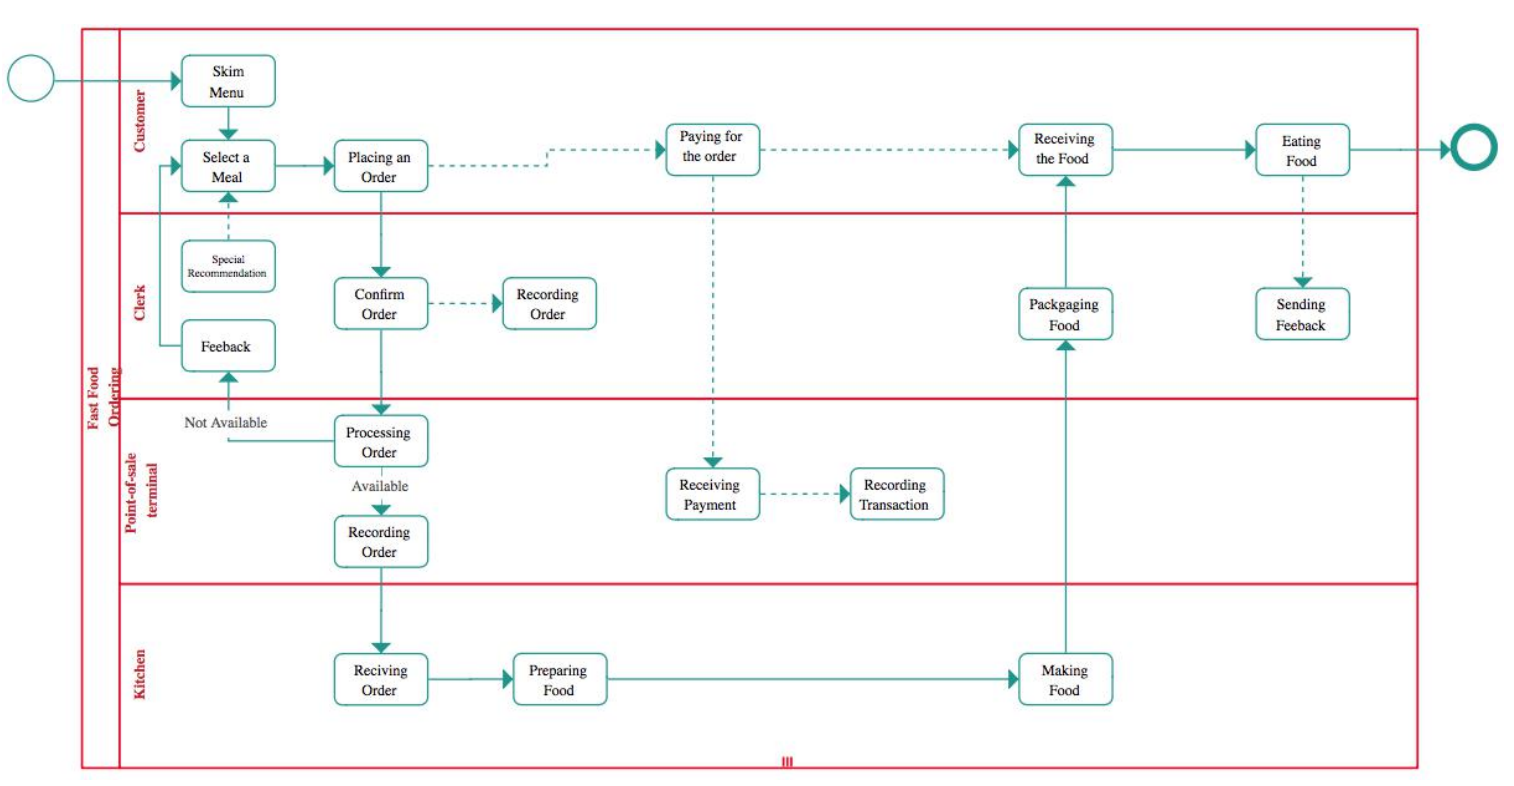
\includegraphics[scale=0.23]{Images/Screenshot from 2021-09-15 23-45-02.png}
    \end{center}
    \caption{Customer-drawing workflow}
\end{figure}

The restaurant owners express several special demands for the new system:

\begin{itemize}
    \item The system should allow non-direct contact between Clerks and Customers.
    \item The system should be implemented using Web technology and QR code, so customers will not have to install apps.
    \item The system should be usable from a mobile device, a tablet device or a normal computer/ laptop.
    \item The system should be extendable to use in multiple restaurants in the future.
    \item The current transactions is about 300 orders per day.
\end{itemize}
\pagebreak

\subsection{Đề xuất}

Với tình trạng dịch bệnh COVID hiện nay, các thành phố đang chuẩn bị mở cưa trờ lại. Cần nhanh chóng có một biện pháp an toàn để cho các cửa hàng thực phẩm trở kinh doanh trở lại mà hạn chế sự tiếp xúc trực tiếp hết mức có thể. Hệ thống POS cho các nhà hàng sẽ là một ứng dụng lý tưởng giúp cho các nhà hàng, quán ăn lớn và trung có thể mau chóng mở cưa kinh doanh trở lại. Ứng dụng sẽ cho phép một khách tự đặt món và thành toán không cần thông qua nhân viên. Nhân viên nhà hàng sẽ tiếp nhận đơn hàng thông qua ứng dụng. Ngoài ra hệ thống sẽ hỗ trợ gửi thông báo bằng FCM hoặc email cho các khách hàng một số thông báo quan trọng.

\subsection{User stories}

Các actor của hệ thống bao gồm: \textit{Customer, Clerk, Chef, Owner, Admin}
\begin{itemize}
    \item Là một Customer, tôi muốn có được điều hướng đến trang đặt món của nhà hàng bằng cách quét mã QR.
    \item Là một Customer, tôi muốn đăng nhập vào hệ thống bằng Oauth hoặc với Username + Password.
    \item Là một Customer, tôi muốn được cung cấp các phương thức thanh toán bằng tài khoản ngân hàng nội địa, visa, paypal, momo, ... 
    \item Là một Customer, tôi muốn có thể thêm, xóa, chỉnh sửa các món ăn với số lượng vào giỏ hàng.
    \item là một Customer, tôi muốn có thể chọn các món trong giỏ hàng và tiến hành đặt đơn hàng.
    \item Là một Customer, tôi muốn có thể mở yêu cầu đặt bàn.
    \item Là một Customer, tôi muốn có thể chỉnh sửa, xóa yêu cầu đặt bàn.
    \item Là một Clerk, tôi muốn có thể phê duyệt hoặc từ chối yêu cầu đặt bàn.
    \item Là một Clerk, tôi muốn có thể thêm, xóa, chỉnh sửa các món ăn với số lượng vào giỏ hàng.
    \item Là một Chef, tôi muốn có thể chuyển trạng thái đơn hàng từ PENDING sang PREPARE hoặc REFUSE.
    \item Là một Clerk, tôi muốn có thể chọn các món trong giỏ hàng và tiến hành đặt đơn hàng cho một khách hàng.
    \item Là một Clerk, tôi muốn có thể chỉnh sưa đơn hàng nếu khách hàng yêu cầu trực tiếp.
    \item Là một Chef, tôi muốn có thể chuyển trạng thái đơn hàng từ REQUEST sang PENDING hoặc REFUSE, từ PENDING sang REFUSE.
    \item Là một Clerk hoặc Chef, tôi muốn có thể gửi thông báo cho Customer nếu có vấn đề về đơn hàng.
    \item Là một Clerk hoặc Chef, tôi có thể ẩn một món ăn trên menu.
    \item Là một Owners, tôi muốn có tất cá chức năng của Clerk, Chef.
    \item Là một OWners, tôi có thể chỉnh sửa thông tin nhà hàng của mình.
    \item Là một Owners, tôi muốn có thể quản lý các bàn có trong nhà hàng của mình.
    \item Là một Owners, tôi có thể xem các thống kê về nhà hàng (doanh thu, doanh số bán ra, so sánh các thông số các món ăn theo các thàng, quý , năm,...).
    \item Là một Owners, tôi có thể tạo ra các menu và lưu lại.
    \item Là một Owners, tôi có thể chọn một trong các menu tồn tại để làm menu cho nhà hàng.
\end{itemize}

%%%%%%%%%%%%%%%%%%%%%%%%%%%%%%%%%%%%
\section{Requirement elicitation}

% \subsection{Task 1.1}

% \begin{itemize}
%     \item The context of this project: Hiện thực hệ thống POS của nhà hàng.
%     \item Stakeholders:
%     \begin{enumerate}
%         \item Chủ nhà hàng, người yêu cầu tạo ra hệ thống và đặt ra các yêu cầu cơ bản cho hệ thống.
%         \item Quản lí nhà hàng, người quản lí nhân viên của nhà hàng.
%         \item Kế toán, người quản lí tài chính của nhà hàng, thống kê doanh thu, lợi nhuận, thu chi của nhà hàng.
%         \item Nhân viên, người phục vụ cho nhà hàng, hướng dẫn khách hàng sử dụng hệ thống.
%         \item Đầu bếp, người tạo ra các món ăn cho nhà hàng.
%         \item Khách hàng, người trực tiếp sử dụng hệ thống để đặt bàn, đặt món ăn, ... 
%     \end{enumerate}
%     \item Expected to be done:
%     \begin{itemize}
%         \item Hệ thống được hoàn thành trước ngày 15/11/2021.
%         \item Hệ thống đáp ứng được các requirements đặt ra.
%         \item Hệ thống có giao diện đẹp, hiệu năng ổn định.
%     \end{itemize}
%     \item The scope of the project: 
%     \begin{itemize}
%         \item Hệ thống có tính năng đặt bàn, đặt món ăn và thanh toán.
%         \item Hệ thống cho phép nhân viên và khách hàng có thể tương tác không trực tiếp với nhau.
%         \item Hệ thống sử dụng công nghệ Web và cho phép quét mã QR để khách hàng không cần phải cài đặt app.
%         \item Hệ thống có thể sử dụng trên điện thoại, tablet và máy tính/laptop.
%         \item Hệ thống có thể mở rộng để dùng cho nhiều nhà hàng trong tương lai.
%         \item Hệ thống đáp ứng được khoảng 300 đơn hàng trên ngày.
%     \end{itemize}
% \end{itemize}

% \subsection{Task 1.2}

\subsection{Functional requirements}

\textbf{Customer requirements}
\begin{itemize}

    \item Hệ thống có thể tạo ra các QR code cho các bàn ăn với nội dung là đường dẫn tới trang đặt món của nhà hàng.
    \item Khách hàng có thể dùng các phần mềm bên thứ 3 để quét các mã qr để lấy đường dẫn tới menu đặt món của nhà hàng.
    \item Khách hàng có thể thanh toán thông qua các api của momo, paypal, ...
    \item Khách hàng có thể tạo ra các đơn hàng.
    \item Khách hàng có thể chỉnh sửa, xóa các đơn hàng chưa được \textit{Clerk} phê chuẩn.
    \item Khách hàng có thể phản hồi, khiếu nại về chất lượng phục vu, đánh giá nhà hàng trên thang điểm 5 sao
    \item Nhận các voucher giảm giá của nhà hàng.
    \item Thông báo cho khách hàng còn chỗ hay không khi khách mở app.
    
\end{itemize}
\textbf{Clerk requirements}
\begin{itemize}
    \item Nhận thực đơn từ khách hàng.
    \item Hệ thống nhận diện khách hàng quen thuộc, nhớ thực đơn yêu thích.
    \item Tạo bảng danh sách các món được ưu thích.
    \item Clerks có thể quản lý các đơn hàng, (hủy, chỉnh sửa, phê duyệt).
    \item Quản lí các khoản nợ của khách.
    \item Giao tiếp được với khách hàng.
    \item Thông báo món làm xong.
\end{itemize}
\textbf{Chef requirements}
\begin{itemize}
    \item Hiển thị thực đơn nấu ăn.
    \item Các yêu cầu về món ăn của từng thực khách.
    \item Đánh dấu món đã xong cho quản lí.
\end{itemize}
 %\includegraphics[scale=0.6]{Images/SE_UML-Functional requirements.drawio (1).png}

\subsection{Non-functional requirements}
\begin{itemize}
    \item Hệ thống có khả năng xử lí 300 đơn hàng trong 1 ngày.
    \item Hệ thống hoạt động ổn định, có khả năng mở rộng, bảo trì và phục hồi
    \item Hệ thống được vận hành trên web và hoạt động 24/7.
\end{itemize}

\newpage
\section{Use-case}
\subsection{System use-case digram}

\begin{figure}[!h]
    \begin{center}
        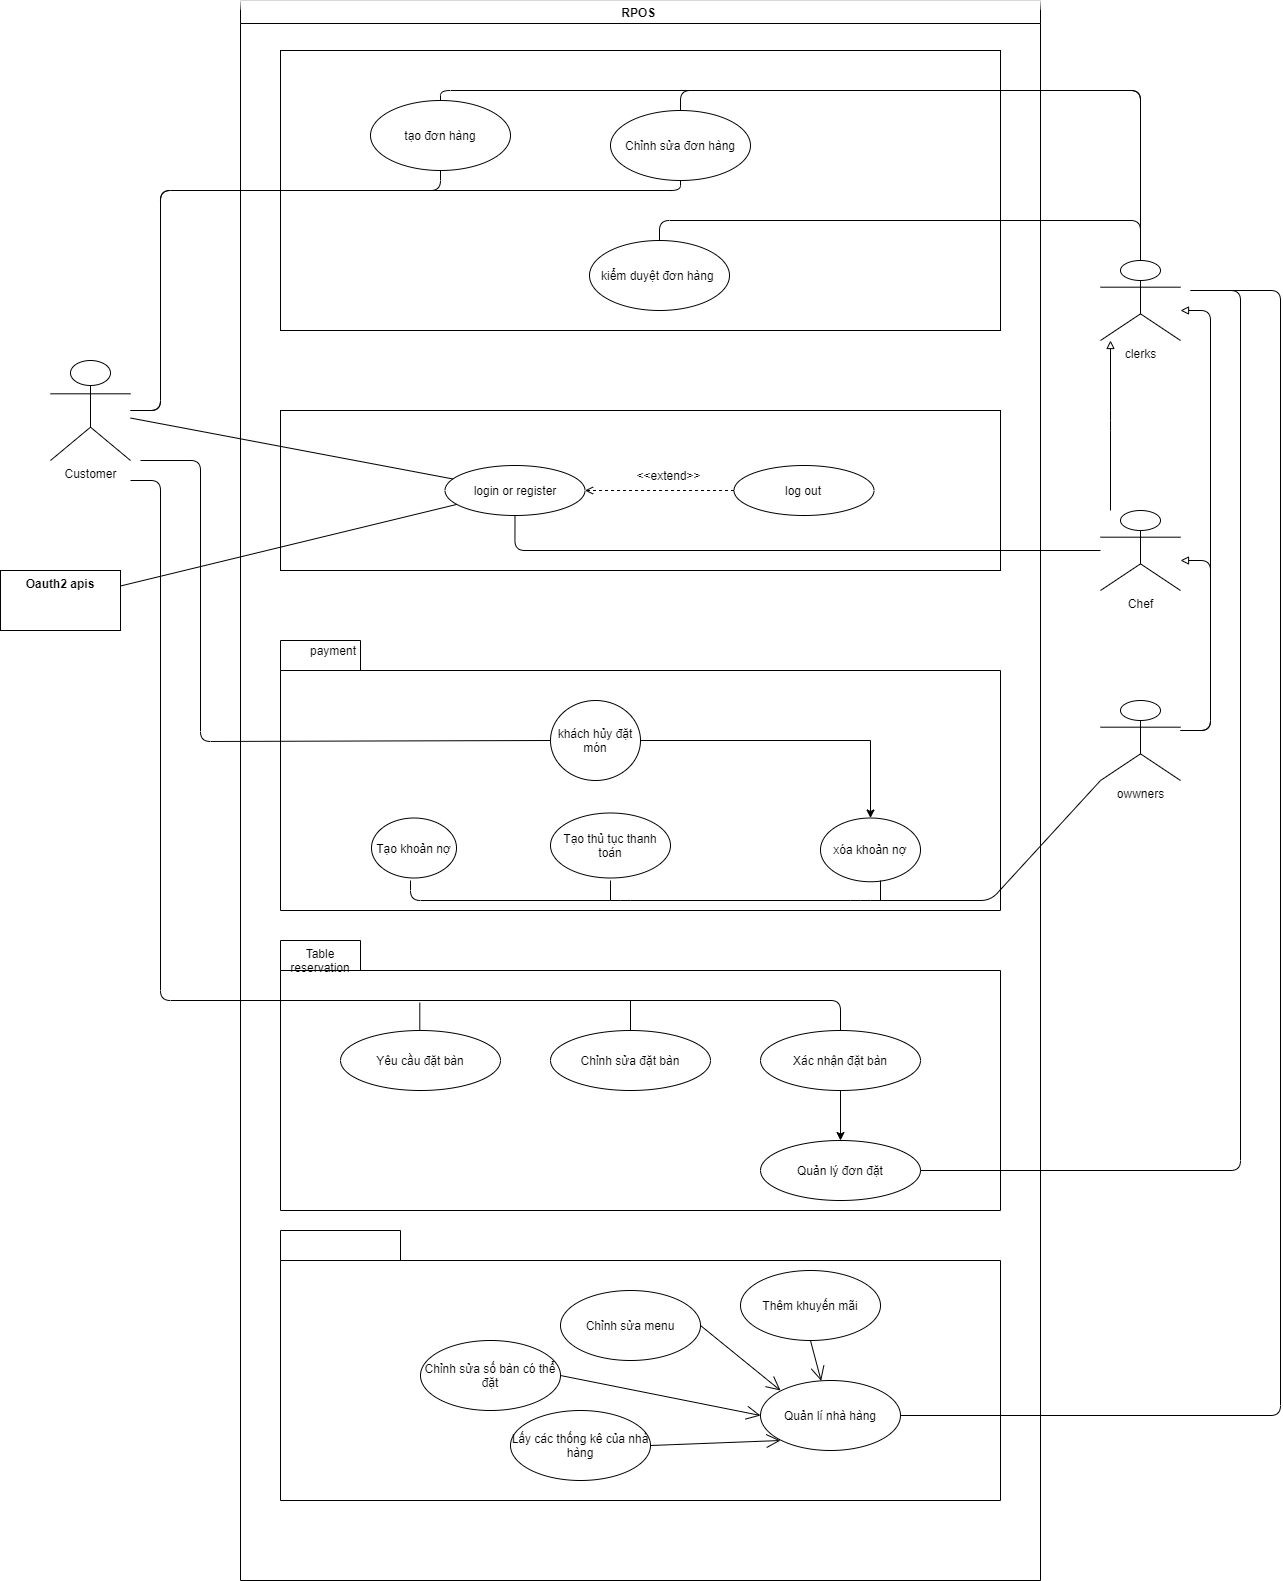
\includegraphics[scale=0.33]{Images/system-use-case.png}
    \end{center}
    \caption{System use-case digram}
\end{figure}

%Chú thích:

% \subsection{System use-case diagram}
% \begin{center}
%     \begin{figure}[!h]
%         \begin{center}
%             \includegraphics[scale=0.5]{Images/Functional requirements.drawio.png} 
%         \end{center}
%         \vspace{1cm}
%         \caption{Authentication use case diagram}
%     \end{figure}
% \end{center}

% \subsubsection{Use-case diagram for the whole system}

\newpage
\subsection{Authenticaition}

\textbf{Use-case diagram}
    \begin{center}
        \begin{figure}[!h]
            \begin{center}
                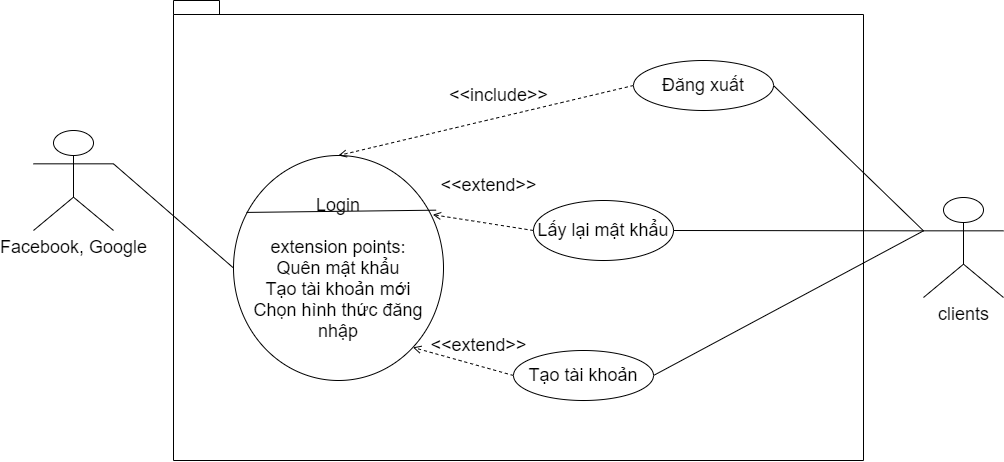
\includegraphics[scale=0.4]{Images/authentication.png} 
            \end{center} 
            \vspace{1cm}
            \caption{Authentication use case diagram}
        \end{figure}    
    \end{center}

\newpage
\begin{enumerate}
    \item Đăng nhập
\begin{center}{\color{black}}

    \begin{tabular}{|p{5cm}|p{7cm}|} \hline
    
        \textbf{Use Case Id} & \textbf{}  \\ \hline
        Tên usecase &  Đăng nhập\\ \hline
        Tiền điều kiện & 
            \begin{enumerate}[1.]                
                \item Tài khoản người dùng đã được tạo sẵn.
                \item Tài khoản người dùng đã được phân quyền.
                \item Thiết bị của người dùng đã được kết nối internet khi thực hiện đăng nhập
            \end{enumerate}\\ \hline
        
        Hậu điều kiện &
            \begin{enumerate}[1.]                
                \item Người dùng đăng nhập ứng dụng thành công.
                \item Hệ thống ghi nhận hoạt động đăng nhập thành công
            \end{enumerate}\\ \hline
        
        Luồng điều kiện chính &  
            \begin{enumerate}[1.]
                \item Người dùng truy cập ứng dụng .
                \item Người dùng chọn phương thức đăng nhập bằng tài khoản 
                \item  Người dùng nhập tài khoản  và chọn lệnh đăng nhập
                \item Hệ thống xác thực thông tin đăng nhập thành công và cho phép người dùng truy cập ứng dụng
                \item Xảy ra lỗi, yêu cầu khác hàng thực hiện lại từ bước 2
                \item Hệ thống ghi nhận hoạt động đăng nhập thành công.
            \end{enumerate}\\
        \hline
        Ngoại lệ &
            \begin{enumerate}[1.]                
                \item Người dùng thoát trang web
                \item Người dùng huỷ phương thức đăng nhập
            \end{enumerate}\\ \hline
        
        Luồng điều kiện phụ & \\ \hline
      
    \end{tabular}
\end{center}
\newpage
\item Đăng kí
\begin{center}{\color{black}}

    \begin{tabular}{|p{5cm}|p{7cm}|} \hline
    
        \textbf{Use Case Id} & \textbf{}  \\ \hline
        Tên usecase &  Đăng kí\\ \hline
        Tiền điều kiện & Người dùng phải có số điện thoại. \\ \hline
        
        Hậu điều kiện &
            \begin{enumerate}[1.]                
                \item Người dùng đăng kí ứng dụng thành công
                \item Hệ thống ghi nhận hoạt động đăng kí thành công
            \end{enumerate}\\ \hline
        
        Luồng điều kiện chính &  
            \begin{enumerate}[1.]
                \item Người dùng truy cập ứng dụng .
                \item Người dùng chọn phương thức đăng kí tài khoản
                \item  Người dùng nhập các thông tin username, password, số điện thoại.
                \item Hệ thống xác thực thông tin đăng kí thành công và cho phép người dùng truy cập ứng dụng
                \item Xảy ra lỗi, yêu cầu khác hàng thực hiện lại từ bước 2
                \item Hệ thống ghi nhận hoạt động đăng nhập thành công.
            \end{enumerate}\\
        \hline
        Ngoại lệ &
            \begin{enumerate}[1.]                
                \item  Người dùng thoát trang web
                \item Người dùng huỷ phương thức đăng kí
            \end{enumerate}\\ \hline
       
        Luồng điều kiện phụ & \\ \hline
      
    \end{tabular}
\end{center}
\newpage
\item Đăng xuất
\begin{center}{\color{black}}

    \begin{tabular}{|p{5cm}|p{7cm}|} \hline
    
        \textbf{Use Case Id} & \textbf{}  \\ \hline
        Tên usecase &  Đăng xuất\\ \hline
        Tiền điều kiện & Người dùng phải đăng nhập vào hệ thống. \\ \hline
        
        Hậu điều kiện &  Người dùng đăng xuất ứng dụng thành công\\ \hline
        Luồng điều kiện chính &  
            \begin{enumerate}[1.]
                \item Người dùng chọn phương thức đăng xuất tài khoản
                \item Hệ thống xác thực thông tin đăng xuất thành công và cho phép người dùng đăng xuất ứng dụng
                \item Xảy ra lỗi, yêu cầu khác hàng thực hiện lại từ bước 1
                \item Hệ thống ghi nhận hoạt động đăng xuất thành công.
            \end{enumerate}\\
        \hline
        Ngoại lệ &
            \begin{enumerate}[1.]                
                \item  Người dùng thoát trang web
                \item Người dùng huỷ phương thức đăng kí
            \end{enumerate}\\ \hline
        
        Luồng điều kiện phụ & \\ \hline
      
    \end{tabular}

\end{center}
\end{enumerate}
\newpage
\subsection{Tạo đơn hàng}

\textbf{Use-case diagram}

\begin{figure}[!h]
    \begin{center}
        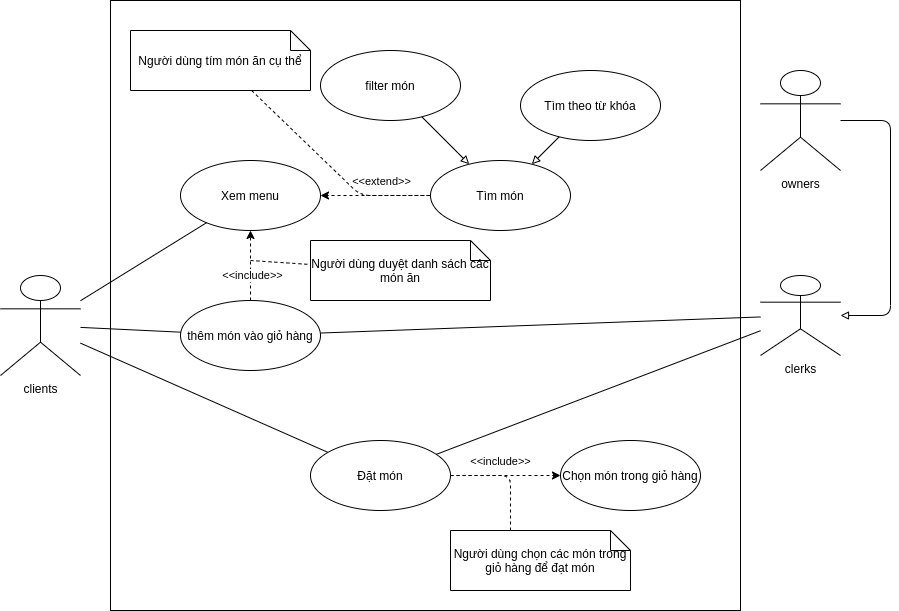
\includegraphics[scale=0.5]{Images/SE_UML-Đặt món.drawio.png}
    \end{center}
    \caption{System use-case digram}
\end{figure}

\newpage
\textbf{Đặc tả use-case}

\begin{center}

    \begin{tabular}{|p{5cm}|p{7cm}|} 
        \hline
        \textbf{Use Case Id} & \textbf{}  \\ \hline
        Tên usecase &  tìm món\\ \hline
        Tiền điều kiện &    \begin{enumerate}
            \item Người dùng nhập từ khóa tìm kiếm hoặc chọn các field để filter.
        \end{enumerate}\\ \hline
        Hậu điều kiện & Trả về danh sách các món phù hợp.\\ \hline
        Luồng điều kiện chính &  
            \begin{enumerate}
                \item Người dùng vào trang menu.
                \item Người dùng nhập từ khóa vào thanh tìm kiếm.
     			\item Người dùng chon search.
            \end{enumerate}\\
        \hline
        Ngoại lệ &  \\ \hline
        Luồng điều kiện phụ &  tại bước 3.
            \begin{enumerate}[start = 3]
                \item[3.b.] Người dùng nhấn chọn tìm kiếm nâng cao.
                \item[4.b.] Người dùng chọn các field trong modal tìm kiếm.
                \item[5.b] Người dùng nhấn tìm kiếm.   
             \end{enumerate}\\
    \hline
    \end{tabular}
\end{center}

\begin{center}{\color{black}}

    \begin{tabular}{|p{5cm}|p{7cm}|} 
        \hline
        \textbf{Use Case Id} & \textbf{}  \\ \hline
        Tên usecase &  thêm món vào giỏ hàng\\ \hline
        Tiền điều kiện &    \begin{enumerate}
            \item Người dùng đã đăng nhập và tài khoản hợp lệ.
        \end{enumerate}\\ \hline
        Hậu điều kiện & Món ăn được thêm vào giỏ hàng\\ \hline
        Luồng điều kiện chính &  
            \begin{enumerate}
                \item Người dùng vào trang menu.
                \item Người dùng chọn món
                \item Nhập số lượng.
				\item Người dùng xác nhận thêm món vào giỏ hàng.
            \end{enumerate}\\
        \hline
        Ngoại lệ &  \\ \hline
        Luồng điều kiện phụ &  \\ \hline
    \end{tabular}
\end{center}

\begin{center}{\color{black}}

    \begin{tabular}{|p{5cm}|p{7cm}|} 
        \hline
        \textbf{Use Case Id} & \textbf{}  \\ \hline
        Tên usecase &  Đặt món\\ \hline
        Tiền điều kiện &    \begin{enumerate}
            \item Người dùng đã đăng nhập và tài khoản hợp lệ.
        \end{enumerate}\\ \hline
        Hậu điều kiện & Đơn hàng mới được thêm vào hệ thống.\\ \hline
        Luồng điều kiện chính &  
            \begin{enumerate}
                \item Người dùng vào giỏ hàng.
                \item Người dùng chọn các món muốn đặt.
				\item Người dùng xác nhận đặt món.
            \end{enumerate}\\
        \hline
        Ngoại lệ &  tại bươc 3 nêu danh sách món được chọn rỗng. Lỗi sẽ được raise lên\\ \hline
        Luồng điều kiện phụ &  tại bước 3 nếu người dùng không phải là Customer.
        \begin{enumerate}
            \item[3.b.] Nhập thông tin khách hàng.
            \item[4.b.] Người dùng xác nhận đặt món.
        \end{enumerate}\\
        \hline
    \end{tabular}
\end{center}

\newpage
\subsection{Chỉnh sửa đơn hàng}

\textbf{Đặc tả}
\begin{center}{\color{black}}

    \begin{tabular}{|p{5cm}|p{7cm}|} \hline
    
        \textbf{Use Case Id} & \textbf{}  \\ \hline
        Tên usecase &   chỉnh sửa đơn hàng\\ \hline
        Tiền điều kiện &    \begin{itemize}
            \item Người dùng đã đăng nhập.
            \item Người dùng là Customer và đơn hàng đang ở trạng thái yêu cầu.
            \item Người dùng là nhân viên nhà hàng và đơn hàng đang ở trạng thái yêu cầu hoặc chờ.
        \end{itemize}\\ \hline
        Hậu điều kiện & \begin{itemize}
            \item Đơn hàng được chỉnh sửa.
        \end{itemize}

        \\ \hline
        Luồng điều kiện chính &  
            \begin{enumerate}
                \item Người dùng chọn một đơn hàng từ danh sách đơn hàng.
                \item Chỉnh sửa đơn hàng (món ăn, số lượng, voucher,...).
				\item Lưu chỉnh sửa.
            \end{enumerate}\\
        \hline
        Ngoại lệ &  \\ \hline
        Luồng điều kiện phụ &  \\ \hline
    \end{tabular}
\end{center}
\newpage
\subsection{Thanh toán}
\subsubsection{Use case UML}
 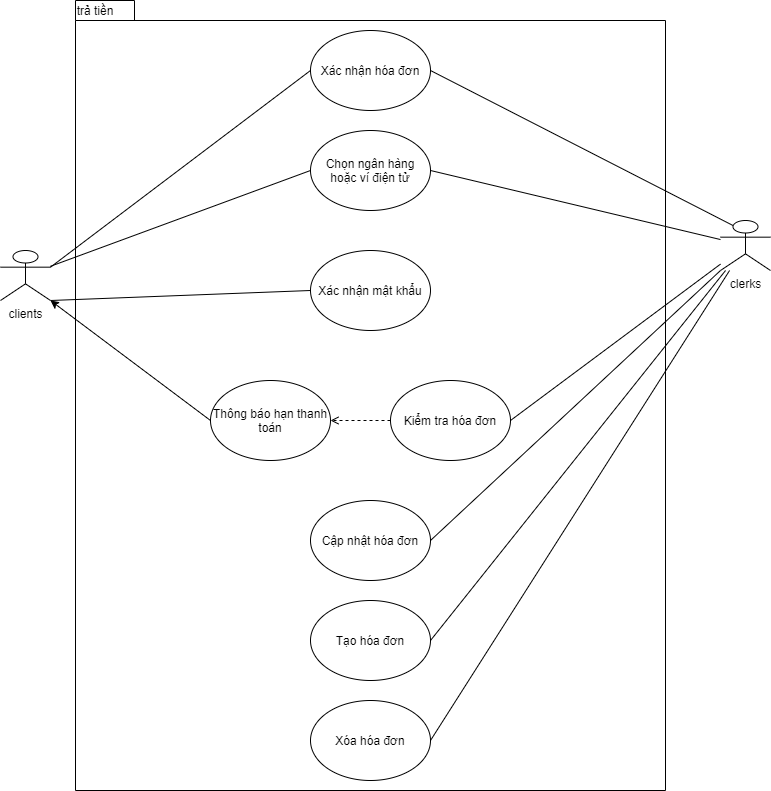
\includegraphics[scale=0.6]{Images/SE_UML-payment.png}

\subsubsection{Dặc tả}
\begin{center}{\color{black}}

    \begin{tabular}{|p{5cm}|p{7cm}|} \hline
    
        \textbf{Use Case Id} & \textbf{}  \\ \hline
        Tên usecase &  Trả tiền\\ \hline
        Tiền điều kiện & Người dùng xác nhận đặt món.\\ \hline
        
        
        Hậu điều kiện &  Người dùng thanh toán khoản nợ.\\ \hline
        Luồng điều kiện chính &  
            \begin{enumerate}
                \item App tạo khoản nợ.
                \item Người dùng yêu cầu thanh toán hóa đơn hoặc quá hạn thanh toán.
                \item App yêu cầu chọn ngân hàng, ví điện tử.
                \item App yêu cầu nhập số tài khoản hoặc quét mã QR.
                \item App yêu cầu xác nhận số tiền.
				\item Xác nhận mật khẩu.
				\item Xác nhận giao dịch.
				\item Xảy ra lỗi, yêu cầu khác hàng thực hiện lại từ bước 4
				\item Thông báo thành công, xóa khoản nợ của khách hàng.
            \end{enumerate}\\
        \hline
        Ngoại lệ & Người dùng hủy thực đơn \\ \hline
        Luồng điều kiện phụ & \\ \hline
      
    \end{tabular}
\end{center}

\newpage
\subsection{Table reservation}
\begin{enumerate}
    \item Use-case diagram
    \begin{center}
        \begin{figure}[!h]
            \begin{center}
                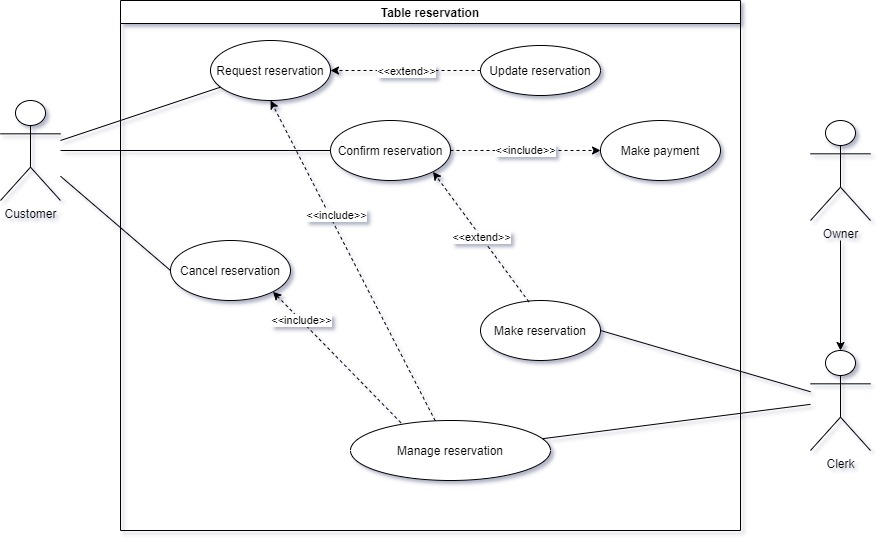
\includegraphics[scale=0.45]{Images/ReservationDiagram.jpg}
            \end{center} 
            \vspace{1cm}
            \caption{Table reservation's use-case diagram}
        \end{figure}    
    \end{center}
    
    \item Use-case make reservation
    \begin{center}{\color{black}}

    \begin{tabular}{|p{5cm}|p{7cm}|} \hline
        Tên usecase &  Request reservation.\\ \hline
        Actor & Khách hàng. \\\hline
        Mô tả & Người dùng sử dụng Request reservation để truy cập ứng dụng web đặt bàn.\\\hline
        Tiền điều kiện & Người dùng phải đăng nhập vào được hệ thống.\\ \hline
        Hậu điều kiện &  Người dùng đã xác nhận đặt bàn và có thông báo được gửi đến.
        \\ \hline
        Luồng điều kiện chính &  
            \begin{enumerate}[1.]
                \item Hệ thống hiển thị giao diện đặt bàn.
                \item Người dùng chọn chức năng  đặt chỗ.
                \item Người dùng xác nhận liệu đó có phải là lần đầu tiên họ ghé thăm nhà hàng.
                
                \item Một biểu mẫu bật lên hỏi người dùng một vài chi tiết cơ bản như tên, chi tiết liên hệ,...
                
			    
            \end{enumerate}\\\hline
        
    \end{tabular}
\end{center}


\begin{center}{\color{black}}

    \begin{tabular}{|p{5cm}|p{7cm}|} \hline
        
        Luồng điều kiện chính &  
            \begin{enumerate}
                \item[5.] Hệ thống hiển thị biểu đồ đặt chỗ ở định dạng bảng (các hàng và cột là thời gian và các ngày trong tuần).
                \item[6.] Người dùng chọn khung thời gian trống và phạm vi giá trong biểu đồ đặt chỗ.
                
				\item[7.] Người dùng đưa ra lựa chọn: Xác nhận/Thay đổi. Nếu xác nhận, hệ thống chuyển sang bước 8. Nếu thay đổi, người dùng thực hiện lại bước 6.
			
				\item[8.] Người dùng tiến hành thanh toán tiền cọc.
				\item[9.] Hệ thống ghi nhận đặt chỗ thành công.
			
            \end{enumerate}\\\hline
        
        Luồng sự kiện phụ &  
                \begin{itemize}
                    \item Thêm chỗ đặt bàn mới.
                    \begin{enumerate}[1.]
                        \item Hệ thống hiển thị giao diện đặt bàn.
                        \item Người dùng chọn khung thời gian phù hợp.
                        \item Người dùng xác nhận thêm chỗ đặt mới.
                    \end{enumerate}
                    \item Xóa chỗ đặt cũ
                    \begin{enumerate}[1.]
                        \item Hệ thống hiển thị các chỗ đặt có thể xóa.
                        \item Người dùng chọn chỗ đặt cần xóa.
                        \item Người dùng xác nhận xóa chỗ đặt
                    \end{enumerate}
                \end{itemize}\\ \hline
    \end{tabular}
\end{center}


    \newpage
    \item Use-case Update reservation
    \begin{center}{\color{black}}
        \begin{tabular}{|p{5cm}|p{7cm}|} \hline
    
        
        Tên usecase &  Update reservation.\\ \hline
        Actor & Khách hàng.\\ \hline
        Mô tả & Người dùng sử dụng Update reservation để truy cập ứng dụng web chỉnh sửa đơn đặt sau khi đã đặt bàn.\\ \hline
        Tiền điều kiện 
        & Người dùng đã đăng nhập vào hệ thống và  đặt bàn  trong vòng 1 giờ.\\ \hline
        
        
        Hậu điều kiện &  Người dùng đã xác nhận  và có thông báo được gửi đến.
                \\ \hline
        Luồng điều kiện chính &  
            \begin{enumerate}[1.]
                \item Người dùng chỉnh sửa các chỗ đã được đặt.
                
                \item Hệ thống hiển thị biểu đồ đặt chỗ. 
                \item Người dùng chọn khung thời gian trống và phạm vi giá trong biểu đồ đặt chỗ hoặc xóa các chỗ đã đặt trước đó.
                
				\item Người dùng đưa ra lựa chọn: Xác nhận/Thay đổi. Nếu xác nhận, hệ thống chuyển sang bước 5. Nếu thay đổi, người dùng thực hiện lại bước 3.
				
				\item Người dùng tiến hành thanh toán tiền cọc.
				\item Hệ thống ghi nhận đặt chỗ thành công.
			
            \end{enumerate}\\
         
        \hline
       
        
    \end{tabular}
    \end{center}




\end{enumerate}


\newpage
\subsection{Restaurant management}
\begin{enumerate}
    \item Use-case diagram:
    \begin{center}
        \begin{figure}[!h]
            \begin{center}
                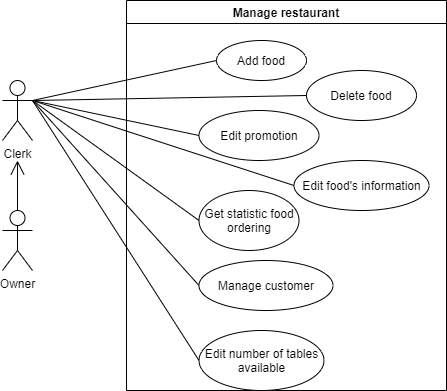
\includegraphics[scale=.5]{Images/managementDiagram.png} 
            \end{center} 
            \vspace{1cm}
            \caption{Restaurant management's use-case diagram}
        \end{figure}    
    \end{center}
    
    \item Use-case "Delete food":
    \begin{center}{\color{black}}
        \begin{tabular}{|p{5cm}|p{7cm}|} \hline
            Tên usecase &   Delete food\\ \hline
            Actor& Clerks \\ \hline
            Mô tả& Use-case cho phép nhân viên có thể xóa món ăn có trong menu \\ \hline
            Tiền điều kiện &    
            \begin{enumerate}[1.]
                \item Nhân viên đã đăng nhập vào hệ thống
                \item Nhân viên chọn chức năng xóa món ăn
            \end{enumerate}\\ \hline
            Hậu điều kiện & Món ăn đã được xóa thành công \\ \hline
            Luồng sự kiện chính &  
                \begin{enumerate}[1.]
                    \item Hệ thống hiển thị màn hình các món ăn có thể xóa.
    				\item Nhân viên chọn món ăn cần xóa.
    				\item Nhân viên chọn hoàn thành
    				\item Hệ thống thông báo đã xóa thành công
    				\item kết thúc use-case
                \end{enumerate}\\
            \hline
        \end{tabular}
    \end{center}
    
    \newpage
    \item Use-case "Add food":
    \begin{center}{\color{black}}
        \begin{tabular}{|p{5cm}|p{7cm}|} \hline
            Tên usecase &   Add food\\ \hline
            Actor& Clerks \\ \hline
            Mô tả& Use-case cho phép nhân viên thêm món ăn mới vào trong menu \\ \hline
            Tiền điều kiện &
            \begin{enumerate}[1.]
                \item Nhân viên đã đăng nhập vào hệ thống
                \item Nhân viên chọn chức năng thêm món ăn
            \end{enumerate}\\ \hline
            Hậu điều kiện & Món ăn mới đã được thêm vào menu\\ \hline
            Luồng sự kiện chính &  
                \begin{enumerate}[1.]
                    \item Hệ thống hiển thị màn hình chứa các thông tin cần điền để mô tả món ăn mới.
                    \item Nhân viên điền các thông tin cần thiết cho món ăn mới.
                    \item Nhân viên xác nhận thông tin món ăn mới và ấn hoàn thành hoặc chọn chỉnh sửa lại.
    				\item kết thúc use-case.
                \end{enumerate} \\\hline
            Luồng sự kiện phụ &
            \begin{enumerate}[1.]
                \item Nhân viên chọn chỉnh sửa lại thông tin món ăn mới.
                \item Nhân viên chỉnh sửa các thông tin món ăn bị sai.
                \item Nhân viên xác nhận thông tin món ăn và ấn hoàn thành.
            \end{enumerate}\\ \hline
        \end{tabular}
    \end{center}
    
    \newpage
    \item Use-case "Edit food'information":
    \begin{center}{\color{black}}
        \begin{tabular}{|p{5cm}|p{7cm}|} \hline
            Tên usecase &   Edit food'information\\ \hline
            Actor& Clerks \\ \hline
            Mô tả& Use-case cho phép nhân viên chỉnh sửa thong tin món ăn trong menu \\ \hline
            Tiền điều kiện &
            \begin{enumerate}[1.]
                \item Nhân viên đã đăng nhập vào hệ thống
                \item Nhân viên chọn chức năng chỉnh sửa món ăn
            \end{enumerate}\\ \hline
            Hậu điều kiện & Thông tin món ăn đã được chỉnh sửa\\ \hline
            Luồng sự kiện chính &  
                \begin{enumerate}[1.]
                    \item Hệ thống hiển thị màn hình chứa các món ăn có thể chỉnh sửa.
                    \item Nhân viên chọn món ăn cần chỉnh sửa.
                    \item Nhân viên chỉnh sửa các thông tin cần thiết cho món ăn.
                    \item Nhân viên xác nhận thông tin món ăn và ấn hoàn thành hoặc chọn chỉnh sửa lại.
    				\item kết thúc use-case.
                \end{enumerate} \\\hline
            Luồng sự kiện phụ &
            \begin{enumerate}[1.]
                \item Nhân viên chọn chỉnh sửa lại thông tin món ăn.
                \item Nhân viên chỉnh sửa các thông tin món ăn bị sai.
                \item Nhân viên xác nhận thông tin món ăn và ấn hoàn thành.
            \end{enumerate}\\ \hline
        \end{tabular}
    \end{center}
    
    \newpage
    \item Use-case "Edit promotion":
    \begin{center}{\color{black}}
        \begin{tabular}{|p{5cm}|p{7cm}|} \hline
            Tên usecase &   Edit promotion\\ \hline
            Actor& Clerks \\ \hline
            Mô tả& Use-case cho phép nhân viên đặt khuyến mãi cho món ăn\\ \hline
            Tiền điều kiện &    
            \begin{enumerate}[1.]
                \item Nhân viên đã đăng nhập vào hệ thống
                \item Nhân viên chọn chức năng thêm khuyến mãi.
            \end{enumerate}\\ \hline
            Hậu điều kiện & Thông tin khuyến mãi của món ăn đã được cập nhật\\ \hline
            Luồng sự kiện chính &  
                \begin{enumerate}[1.]
                    \item Hệ thống hiển thị màn hình các món ăn có thể đặt khuyến mãi.
    				\item Nhân viên chọn món ăn cần đặt khuyến mãi.
    				\item Nhân viên đặt giá khuyến mãi hoặc phần trăm khuyến mãi cho món ăn.
    				\item Nhân viên chọn hoàn thành
    				\item Hệ thống thông báo đã đặt khuyến mãi thành công.
    				\item kết thúc use-case
                \end{enumerate}\\
            \hline
        \end{tabular}
    \end{center}
    
    \item Use-case "get statistic food ordering":
    \begin{center}{\color{black}}
        \begin{tabular}{|p{5cm}|p{7cm}|} \hline
            Tên usecase &  Get statistic food ordering\\ \hline
            Actor& Clerks \\ \hline
            Mô tả& Use-case cho phép nhân viên thống kê về các đơn hàng đã được thực hiện \\ \hline
            Tiền điều kiện &
            \begin{enumerate}[1.]
                \item Nhân viên đã đăng nhập vào hệ thống
                \item Nhân viên chọn chức năng lấy thống kê đơn hàng
            \end{enumerate}\\ \hline
            Hậu điều kiện &     Người dùng biết được thống kê các đơn hàng đã được thực hiện\\ \hline
            Luồng sự kiện chính &  
                \begin{enumerate}[1.]
                    \item Hệ thống hiển thị màn hình chứa các thống kê về số lượng các đơn hàng, tổng thu, thông tin cụ thể các đơn hàng.
    				\item kết thúc use-case
                \end{enumerate} \\\hline
        \end{tabular}
    \end{center}
    
    \item Use-case "Manage customer":
    \begin{center}{\color{black}}
        \begin{tabular}{|p{5cm}|p{7cm}|} \hline
            Tên usecase & Manager customer\\ \hline
            Actor& Clerks \\ \hline
            Mô tả& Use-case cho phép nhân viên thống kê các thông tin về các khách hàng \\ \hline
            Tiền điều kiện &
            \begin{enumerate}[1.]
                \item Nhân viên đã đăng nhập vào hệ thống
                \item Nhân viên chọn chức năng quản lí khách hàng.
            \end{enumerate}\\ \hline
            Hậu điều kiện & Nhân viên biết được các thông tin về các khách hàng \\ \hline
            Luồng sự kiện chính &  
                \begin{enumerate}[1.]
                    \item Hệ thống hiển thị màn hình chứa các thông tin về số lượng các khách hàng của hệ thống, các thông tin của từng khách hàng.
    				\item kết thúc use-case
                \end{enumerate} \\\hline
        \end{tabular}
    \end{center}
    
    \item Use-case edit number of tables available:
    \begin{center}{\color{black}}
        \begin{tabular}{|p{5cm}|p{7cm}|} \hline
            Tên usecase &   Edit number of tables available\\ \hline
            Actor& Clerks \\ \hline
            Mô tả& Use-case cho phép nhân viên chỉnh sửa số bàn có thể đặt giữ chỗ của nhà hàng\\ \hline
            Tiền điều kiện &
            \begin{enumerate}[1.]
                \item Nhân viên đã đăng nhập vào hệ thống
                \item Nhân viên chọn chức năng chỉnh sửa số bàn dành cho đặt trước.
            \end{enumerate}\\ \hline
            Hậu điều kiện &     Nhân viên cài đặt số bàn có thể đặt thành công \\ \hline
            Luồng sự kiện chính &  
                \begin{enumerate}[1.]
                    \item Hệ thống hiển thị màn hình chỉnh sửa số bàn mà khách có thể giữ chỗ
                    \item Nhân viên nhập số bàn: Bàn vip, bàn cho gia đình, bàn cho couple. 
                    \item Nhân viên chọn chọn hoàn thành
    				\item kết thúc use-case
                \end{enumerate} \\\hline
        \end{tabular}
    \end{center}
\end{enumerate}

\newpage
\section{Activity Diagram}
\subsection{Đăng nhập, đăng ký, đăng xuất}

\begin{figure}[!h]
    \begin{center}
        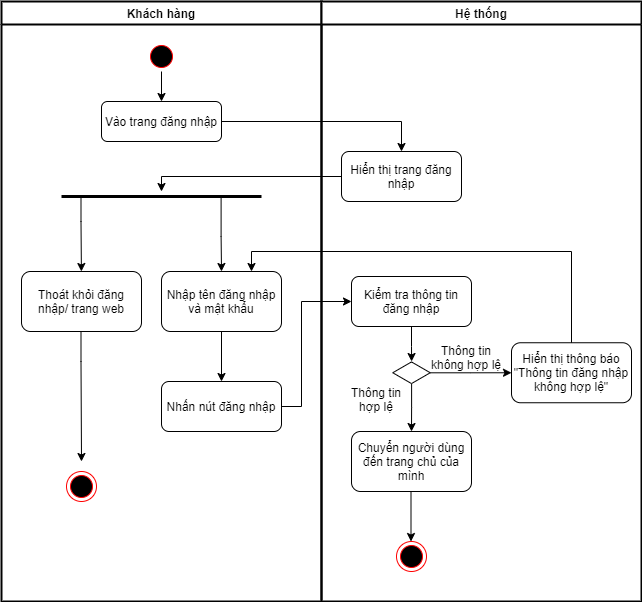
\includegraphics[scale=0.6]{Images/ActivityDiagram/login.drawio.png}
    \end{center}
    \hspace{0.3cm}
    \caption{Đăng nhập}
\end{figure}

\newpage

\begin{figure}[!h]
    \begin{center}
        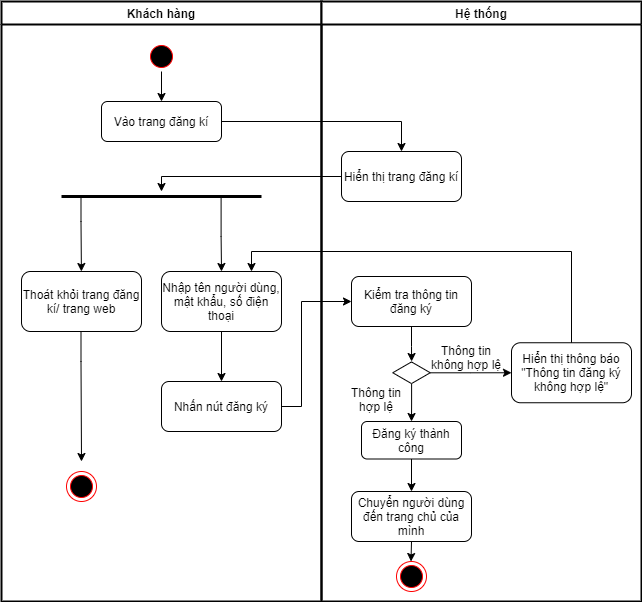
\includegraphics[scale=0.6]{Images/ActivityDiagram/register.drawio.png}
    \end{center}
    \hspace{0.3cm}
    \caption{Đăng ký}
\end{figure}

\newpage

\begin{figure}[!h]
    \begin{center}
        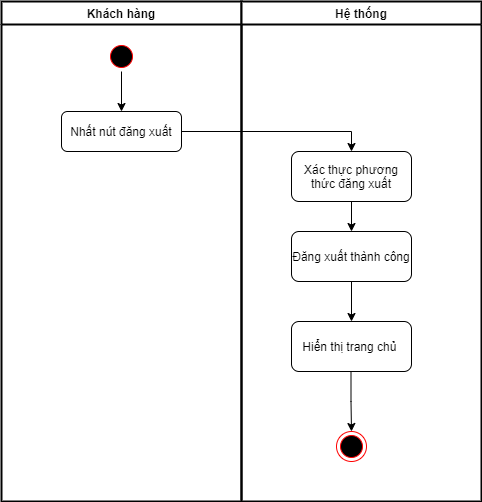
\includegraphics[scale=0.7]{Images/ActivityDiagram/logout.drawio.png}
    \end{center}
    \hspace{0.3cm}
    \caption{Đăng xuất}
\end{figure}
\newpage
\subsection{Đặt bàn, phê duyệt bàn đã đặt}

\begin{figure}[!h]
    \begin{center}
        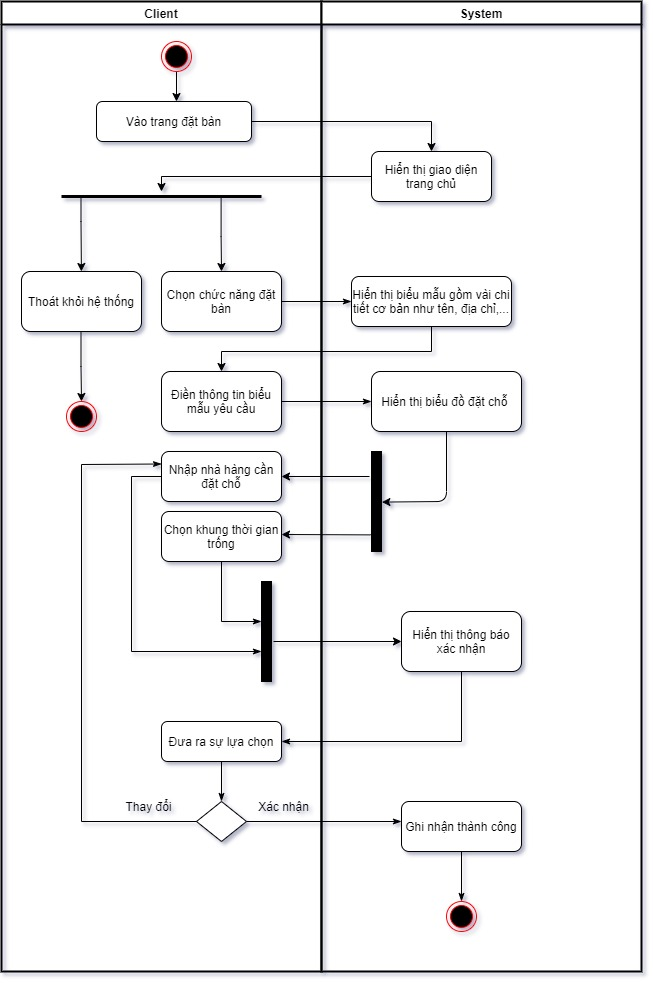
\includegraphics[scale=0.5]{Images/ActivityDiagram/booking_ad.jpg}
    \end{center}
    \hspace{0.3cm}
    \caption{Đặt bàn}
\end{figure}

\newpage

\begin{figure}[!h]
    \begin{center}
        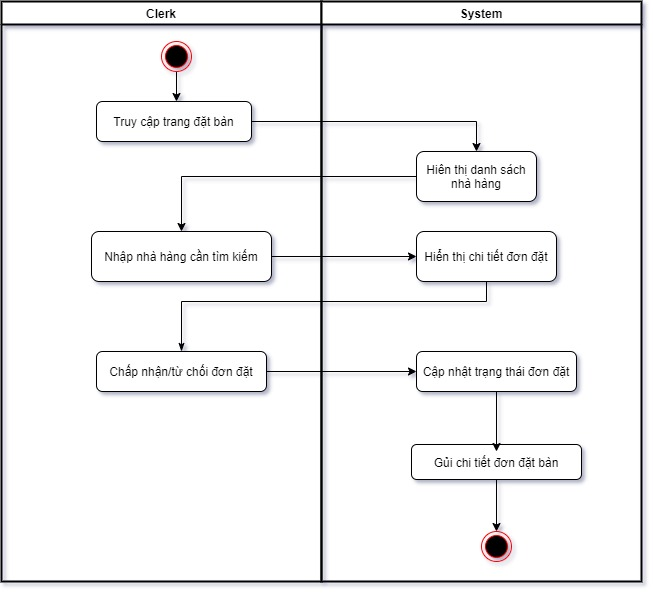
\includegraphics[scale=0.6]{Images/ActivityDiagram/pheduyetBooking_ad.jpg}
    \end{center}
    \hspace{0.3cm}
    \caption{Phê duyệt bàn đã đặt}
\end{figure}


\newpage
\subsection{Thêm món vào giỏ hàng, đặt món, phê duyệt món}

\begin{figure}[!h]
    \begin{center}
        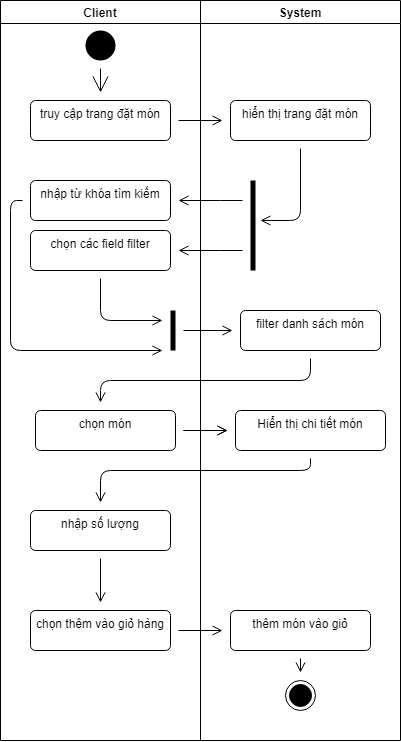
\includegraphics[scale=0.6]{Images/ActivityDiagram/addToCart.png}
    \end{center}
    \hspace{0.3cm}
    \caption{Thêm món vào giỏ hàng}
\end{figure}

\newpage

\begin{figure}[!h]
    \begin{center}
        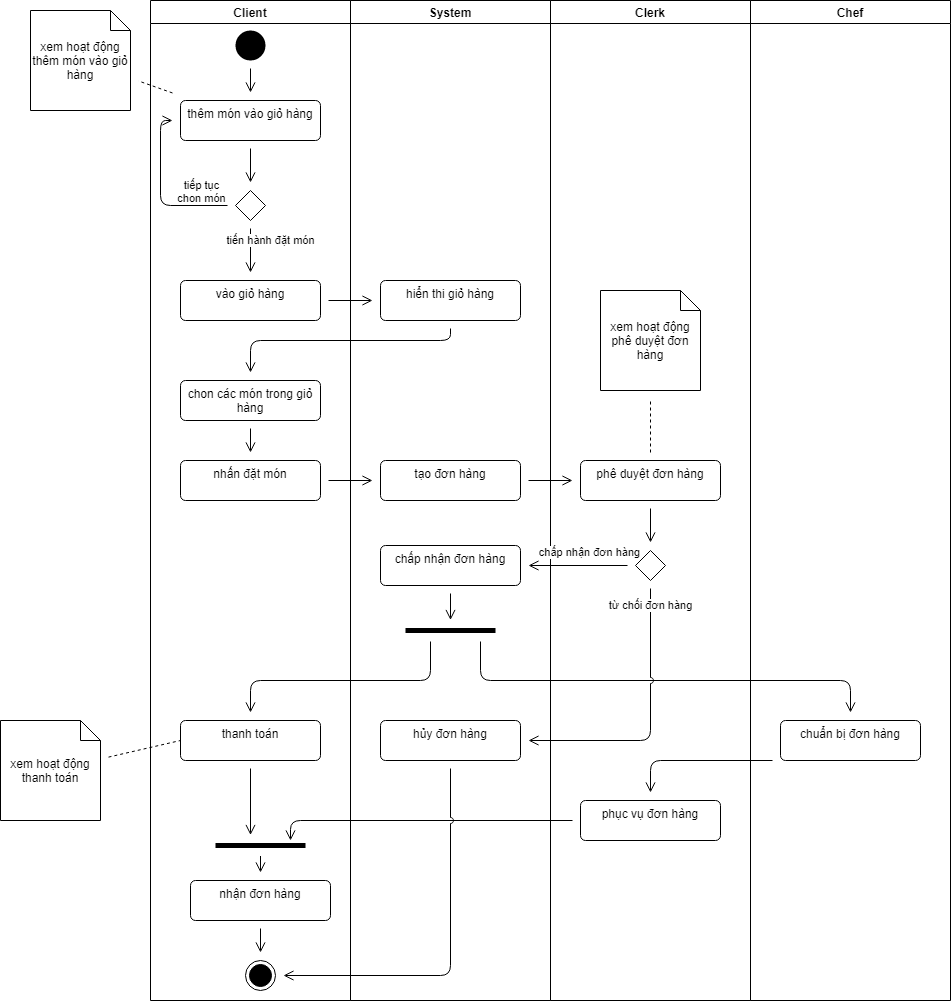
\includegraphics[scale=0.4]{Images/ActivityDiagram/order.png}
    \end{center}
    \hspace{0.3cm}
    \caption{Đặt món}
\end{figure}

\newpage

\begin{figure}[!h]
    \begin{center}
        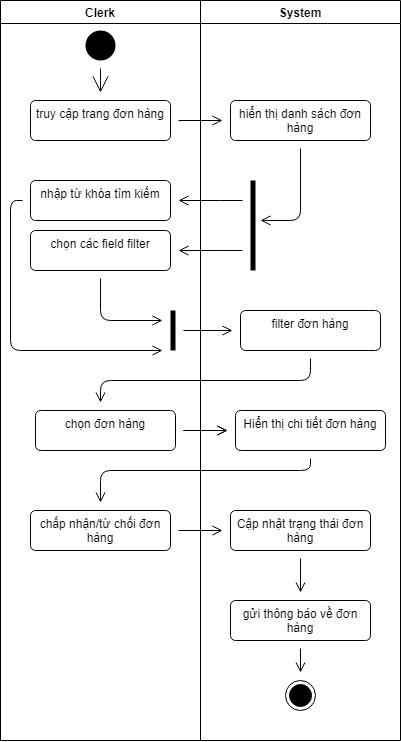
\includegraphics[scale=0.7]{Images/ActivityDiagram/processingOrder.png}
    \end{center}
    \hspace{0.3cm}
    \caption{Phê duyệt đơn hàng}
\end{figure}
\newpage
\subsection{Quản lí nhà hàng}
\begin{figure}[!h]
    \begin{center}
        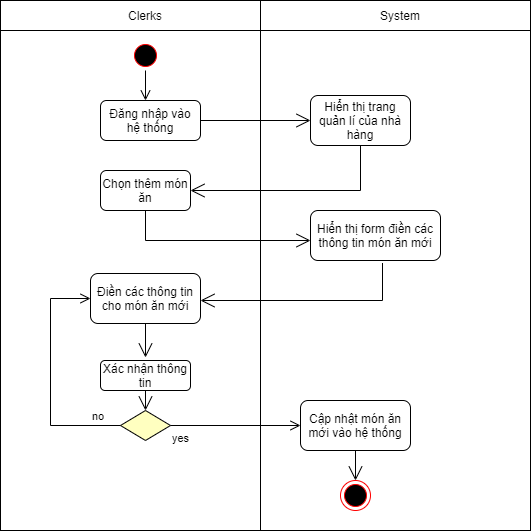
\includegraphics[scale=0.45]{Images/ActivityDiagram/AD_add.png}
    \end{center}
    \hspace{0.3cm}
    \caption{Thêm món ăn vào Menu}
\end{figure}
\begin{figure}[!h]
    \begin{center}
        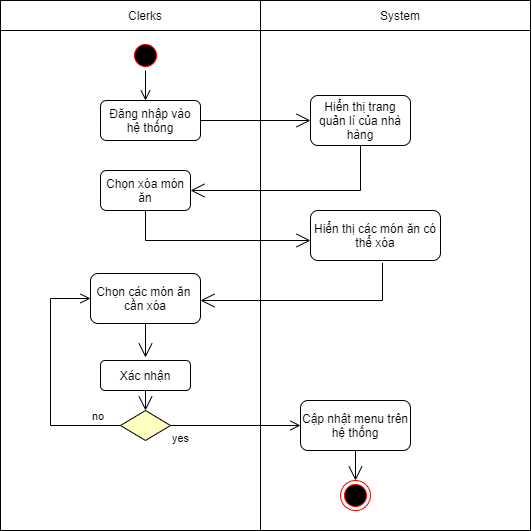
\includegraphics[scale=0.45]{Images/ActivityDiagram/AD_delete.png}
    \end{center}
    \hspace{0.3cm}
    \caption{Xóa món ăn khỏi Menu}
\end{figure}
\newpage
\begin{figure}[!h]
    \begin{center}
        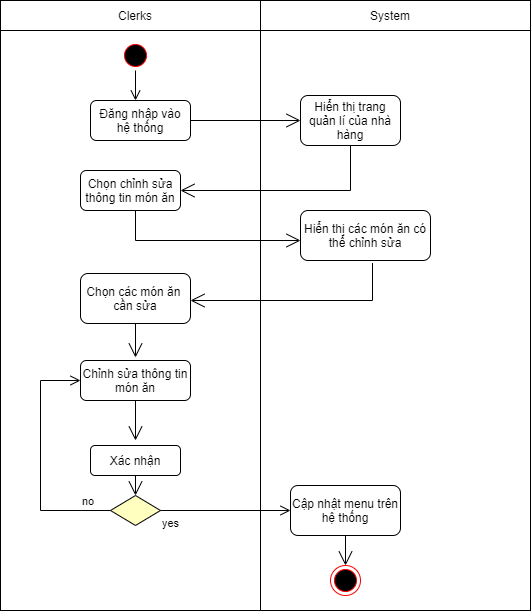
\includegraphics[scale=0.4]{Images/ActivityDiagram/AD_edit.png}
    \end{center}
    \hspace{0.2cm}
    \caption{Chỉnh sửa thông tin món ăn}
\end{figure}
\begin{figure}[!h]
    \begin{center}
        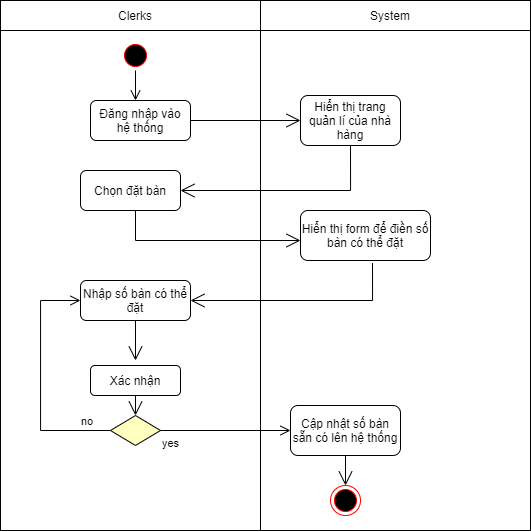
\includegraphics[scale=0.45]{Images/ActivityDiagram/AD_tables.png}
    \end{center}
    \hspace{0.2cm}
    \caption{Chỉnh sửa số bàn đặt trước}
\end{figure}
\newpage
\begin{figure}[!h]
    \begin{center}
        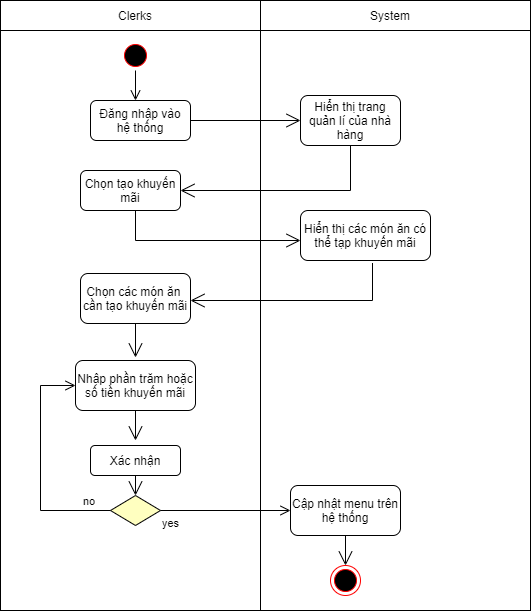
\includegraphics[scale=0.5]{Images/ActivityDiagram/AD_promotion.png}
    \end{center}
    \hspace{0.3cm}
    \caption{Tạo khuyến mãi}
\end{figure}
\begin{figure}[!h]
    \begin{center}
        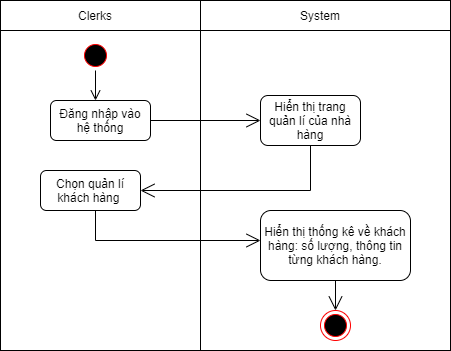
\includegraphics[scale=0.4]{Images/ActivityDiagram/AD_customers.png}
    \end{center}
    \hspace{0.3cm}
    \caption{Quản lí khách hàng}
\end{figure}
\begin{figure}[!h]
    \begin{center}
        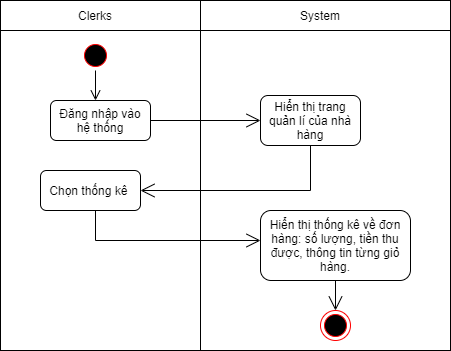
\includegraphics[scale=0.5]{Images/ActivityDiagram/AD_statistic.png}
    \end{center}
    \hspace{0.3cm}
    \caption{Quản lí đơn hàng}
\end{figure}

\newpage
\section{Sequence Diagram}
\subsection{Đăng nhập, đăng ký, đăng xuất}

\begin{figure}[!h]
    \begin{center}
        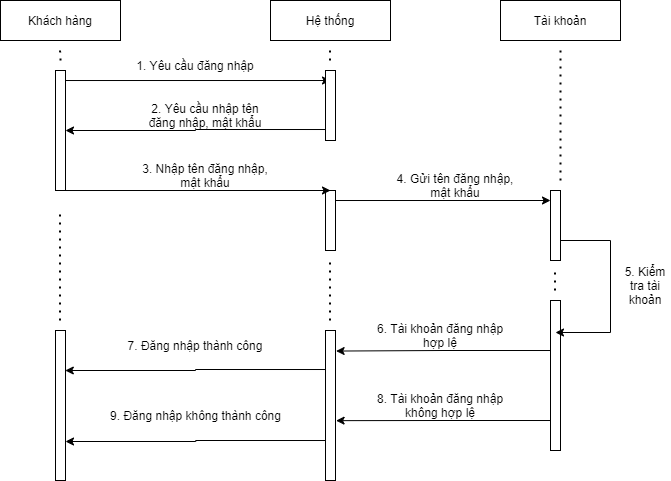
\includegraphics[scale=0.6]{Images/SequenceDiagram/s_login.drawio.png}
    \end{center}
    \hspace{0.3cm}
    \caption{Đăng nhập}
\end{figure}

\newpage

\begin{figure}[!h]
    \begin{center}
        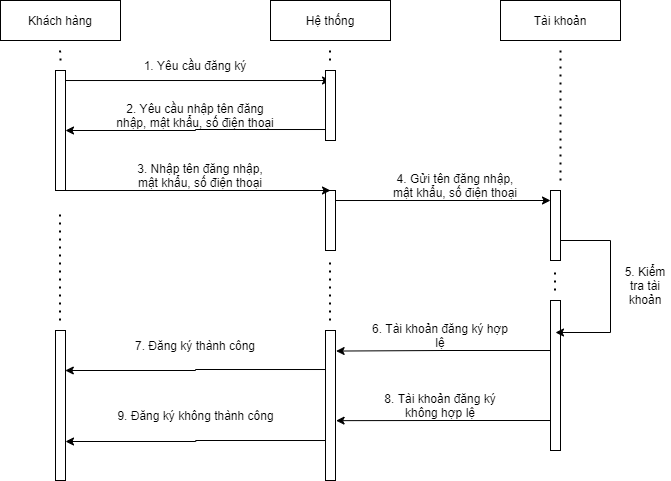
\includegraphics[scale=0.6]{Images/SequenceDiagram/s_register.drawio.png}
    \end{center}
    \hspace{0.3cm}
    \caption{Đăng ký}
\end{figure}

\begin{figure}[!h]
    \begin{center}
        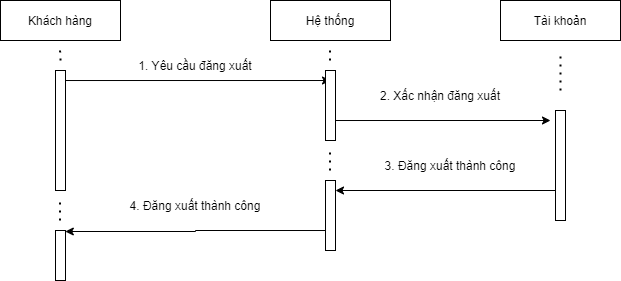
\includegraphics[scale=0.7]{Images/SequenceDiagram/s_logout.drawio.png}
    \end{center}
    \hspace{0.3cm}
    \caption{Đăng xuất}
\end{figure}
\subsection{Thêm món vào giỏ hàng, đặt món, phê duyệt món}

\begin{figure}[!h]
    \begin{center}
        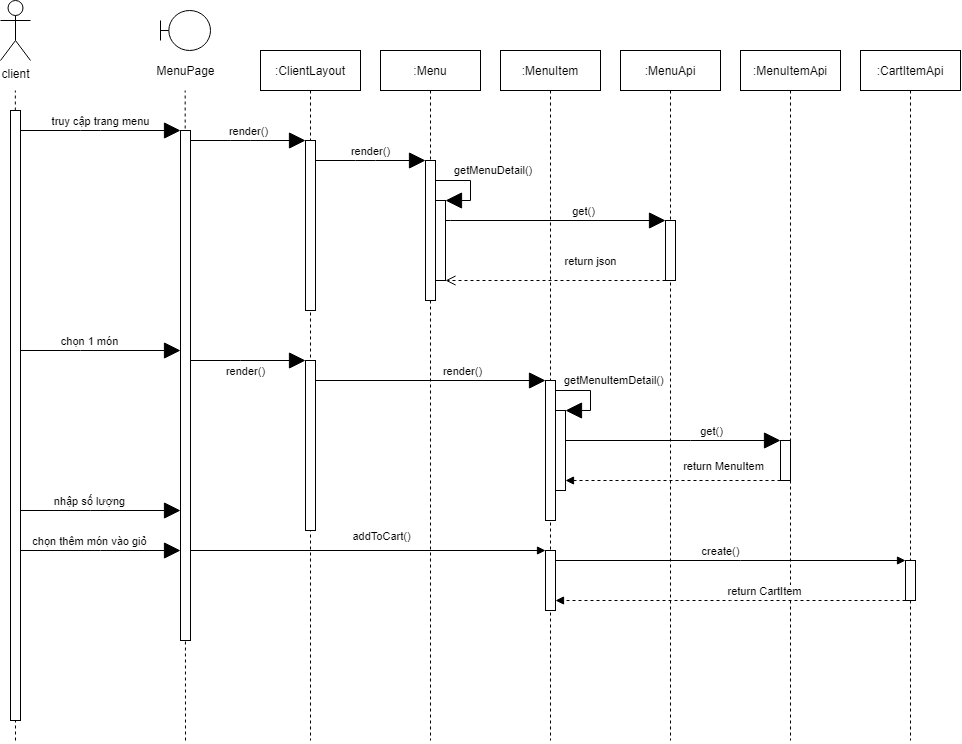
\includegraphics[scale=0.4]{Images/SequenceDiagram/insertToCart.png}
    \end{center}
    \hspace{0.3cm}
    \caption{Thêm món vào giỏ hàng}
\end{figure}

\newpage

\begin{figure}[!h]
    \begin{center}
        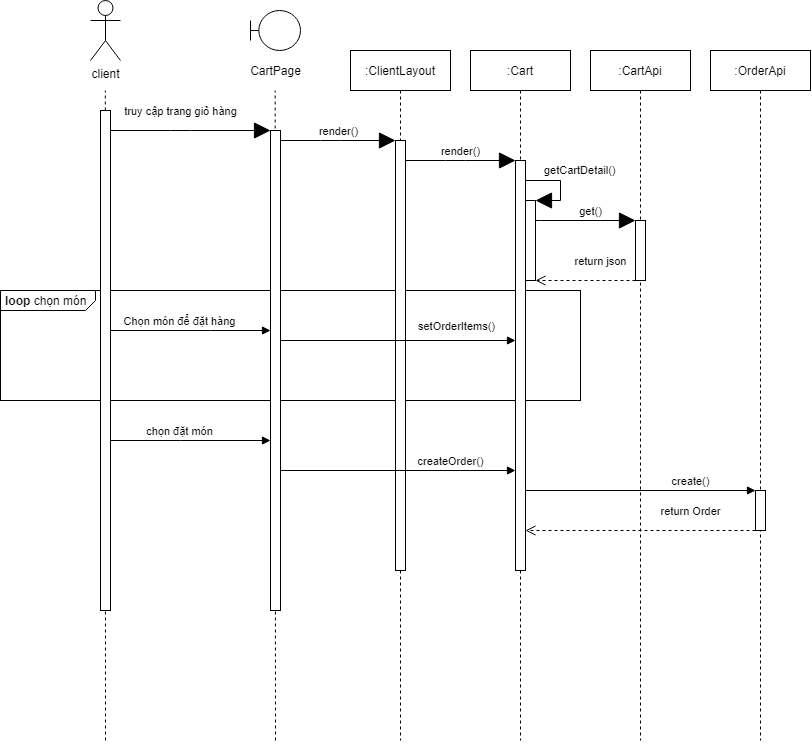
\includegraphics[scale=0.5]{Images/SequenceDiagram/makeOrder.png}
    \end{center}
    \hspace{0.3cm}
    \caption{Đặt món}
\end{figure}

\newpage

\begin{figure}[!h]
    \begin{center}
        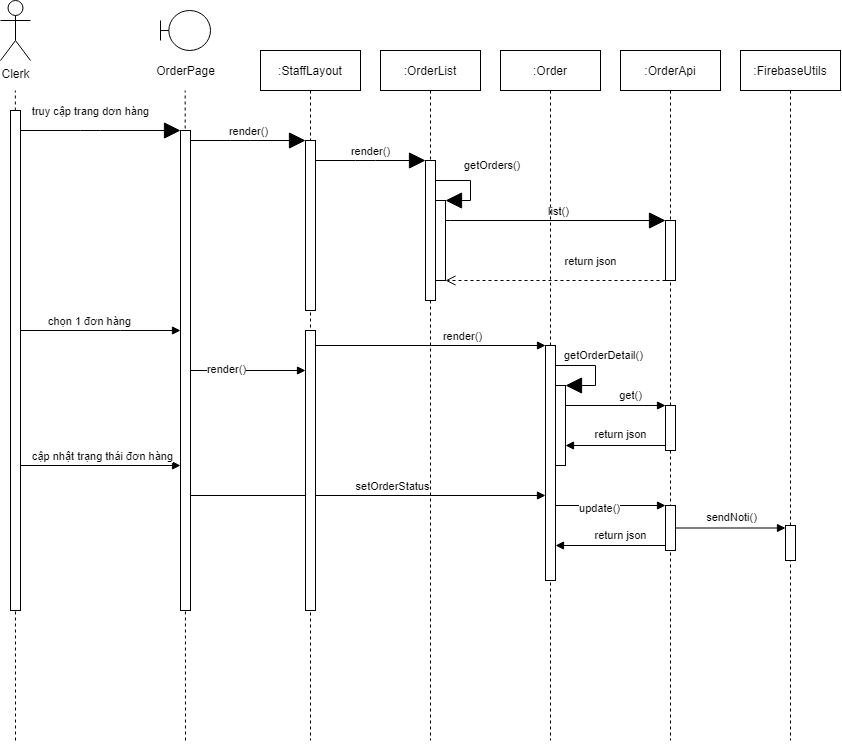
\includegraphics[scale=0.45]{Images/SequenceDiagram/OrderStatus.png}
    \end{center}
    \hspace{0.3cm}
    \caption{Phê duyệt đơn hàng}
\end{figure}
\newpage

\subsection{Đặt bàn}



\begin{figure}[!h]
    \begin{center}
        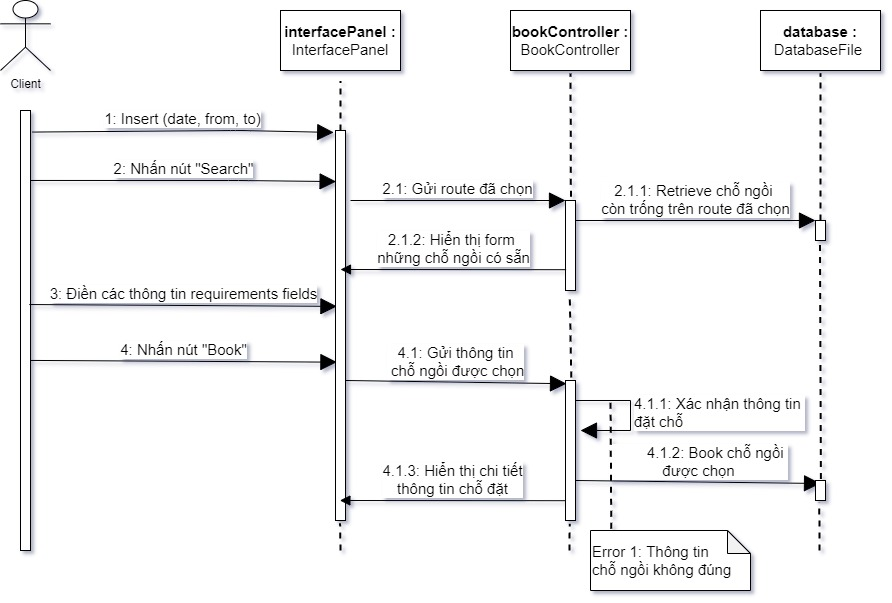
\includegraphics[scale=0.5]{Images/SequenceDiagram/booking_sd.jpg}
    \end{center}
    \hspace{0.3cm}
    \caption{Đặt bàn}
\end{figure}


\newpage
\subsection{Thanh toán}

\begin{figure}[!h]
    \begin{center}
        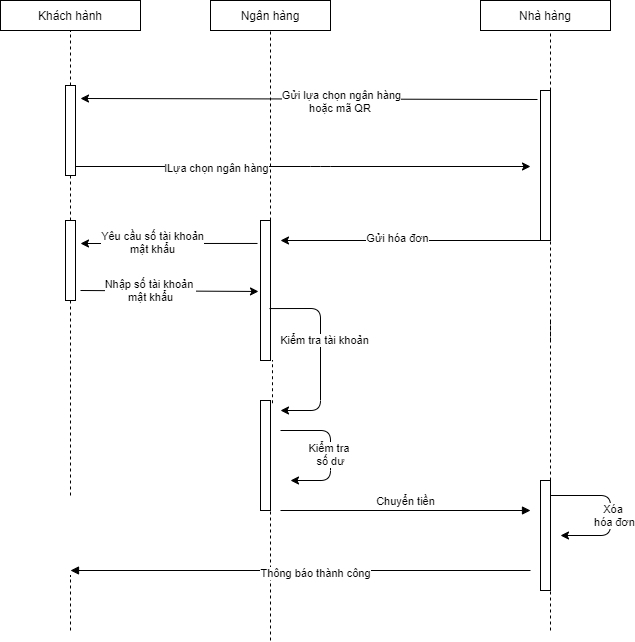
\includegraphics[scale=0.6]{Images/SequenceDiagram/SE_UML-SequencePayment.drawio.png}
    \end{center}
    \hspace{0.3cm}
    \caption{Thanh toán}
\end{figure}

\subsection{Quản lí nhà hàng}
\begin{figure}[!h]
    \begin{center}
        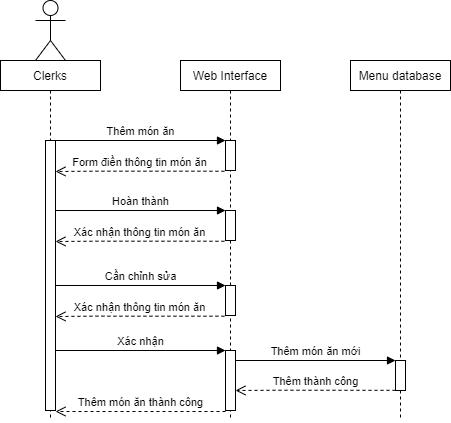
\includegraphics[scale=0.6]{Images/SequenceDiagram/SD_add.png}
    \end{center}
    \hspace{0.3cm}
    \caption{Thêm món ăn vào menu}
\end{figure}
\begin{figure}[!h]
    \begin{center}
        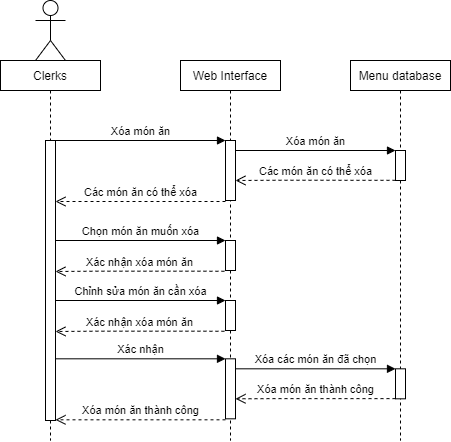
\includegraphics[scale=0.6]{Images/SequenceDiagram/SD_delete.png}
    \end{center}
    \hspace{0.3cm}
    \caption{Xóa món ăn khỏi menu}
\end{figure}
\newpage
\begin{figure}[!h]
    \begin{center}
        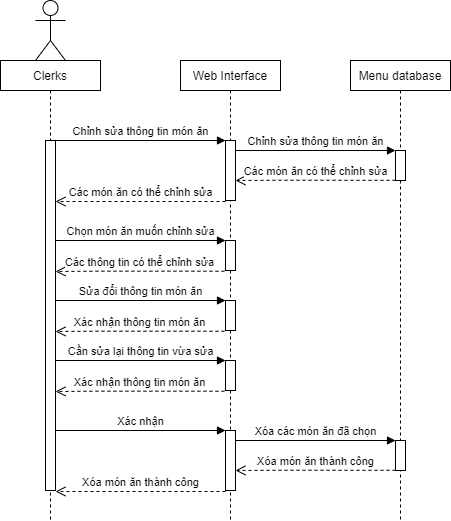
\includegraphics[scale=0.6]{Images/SequenceDiagram/SD_edit.png}
    \end{center}
    \hspace{0.3cm}
    \caption{Chỉnh sửa thông tin món ăn}
\end{figure}
\begin{figure}[!h]
    \begin{center}
        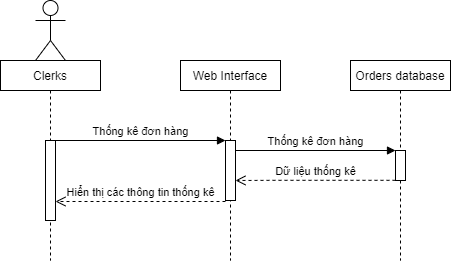
\includegraphics[scale=0.5]{Images/SequenceDiagram/SD_statistic.png}
    \end{center}
    \hspace{0.3cm}
    \caption{Thống kê đơn hàng}
\end{figure}
\newpage
\begin{figure}[!h]
    \begin{center}
        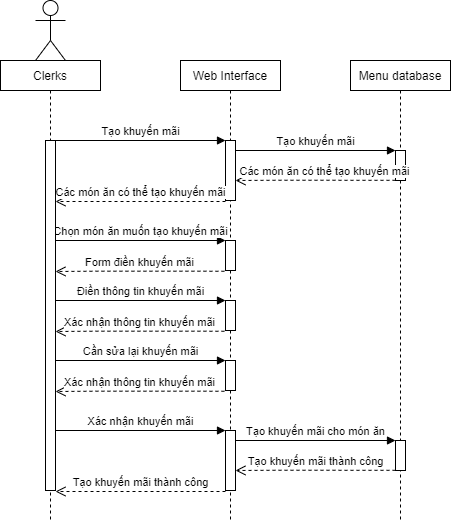
\includegraphics[scale=0.6]{Images/SequenceDiagram/SD_promotion.png}
    \end{center}
    \hspace{0.3cm}
    \caption{Tạo khuyến mãi}
\end{figure}
\begin{figure}[!h]
    \begin{center}
        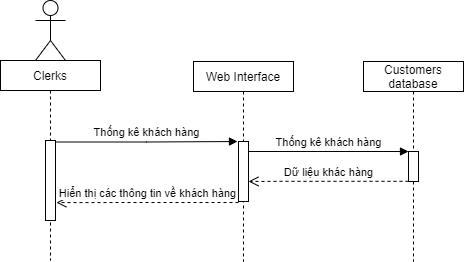
\includegraphics[scale=0.5]{Images/SequenceDiagram/SD_customers.png}
    \end{center}
    \hspace{0.3cm}
    \caption{Thống kê khách hàng}
\end{figure}

\begin{figure}[!h]
    \begin{center}
        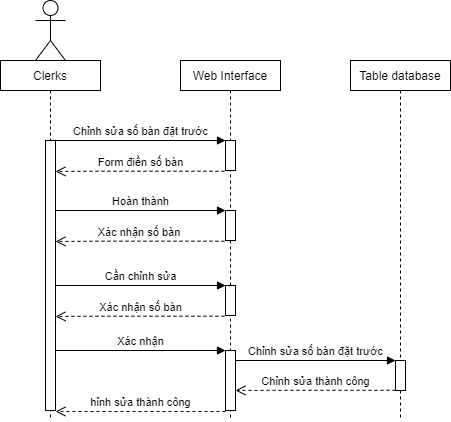
\includegraphics[scale=0.5]{Images/SequenceDiagram/SD_table.png}
    \end{center}
    \hspace{0.3cm}
    \caption{Chỉnh sửa số bàn đặt trước}
\end{figure}


\newpage
\section{Class Diagram}

Vì sẽ khó để quan sát khi chỉ có một class diagram chung cho hệ thống  nên nhóm đã quyết định sẽ dùng một entity class digram chung cho hệ thống và các chức năng sẽ có class diagram riêng.

\subsection{Entity class diagram}

\begin{figure}[!h]
    \begin{center}
        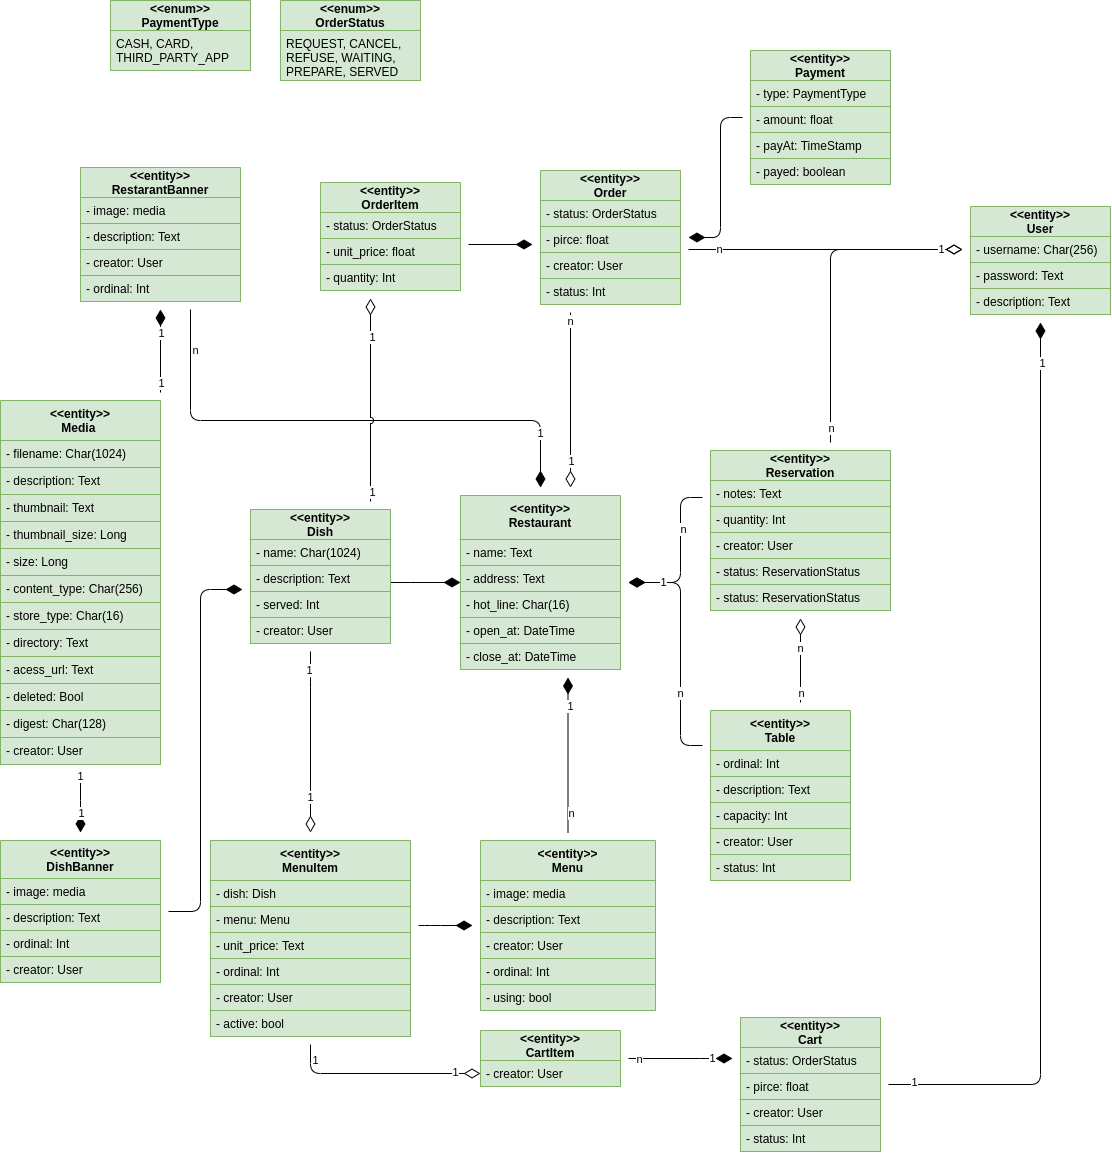
\includegraphics[scale=0.4]{Images/ClassDiagram/entity.png}
    \end{center}
    \hspace{0.3cm}
    \caption{entity class diagram}
\end{figure}
\newpage
\subsection{Thêm món vào giỏ, đặt món, phê duyệt đơn hàng}
\subsubsection{Diagram}
\begin{figure}[!h]
    \begin{center}
        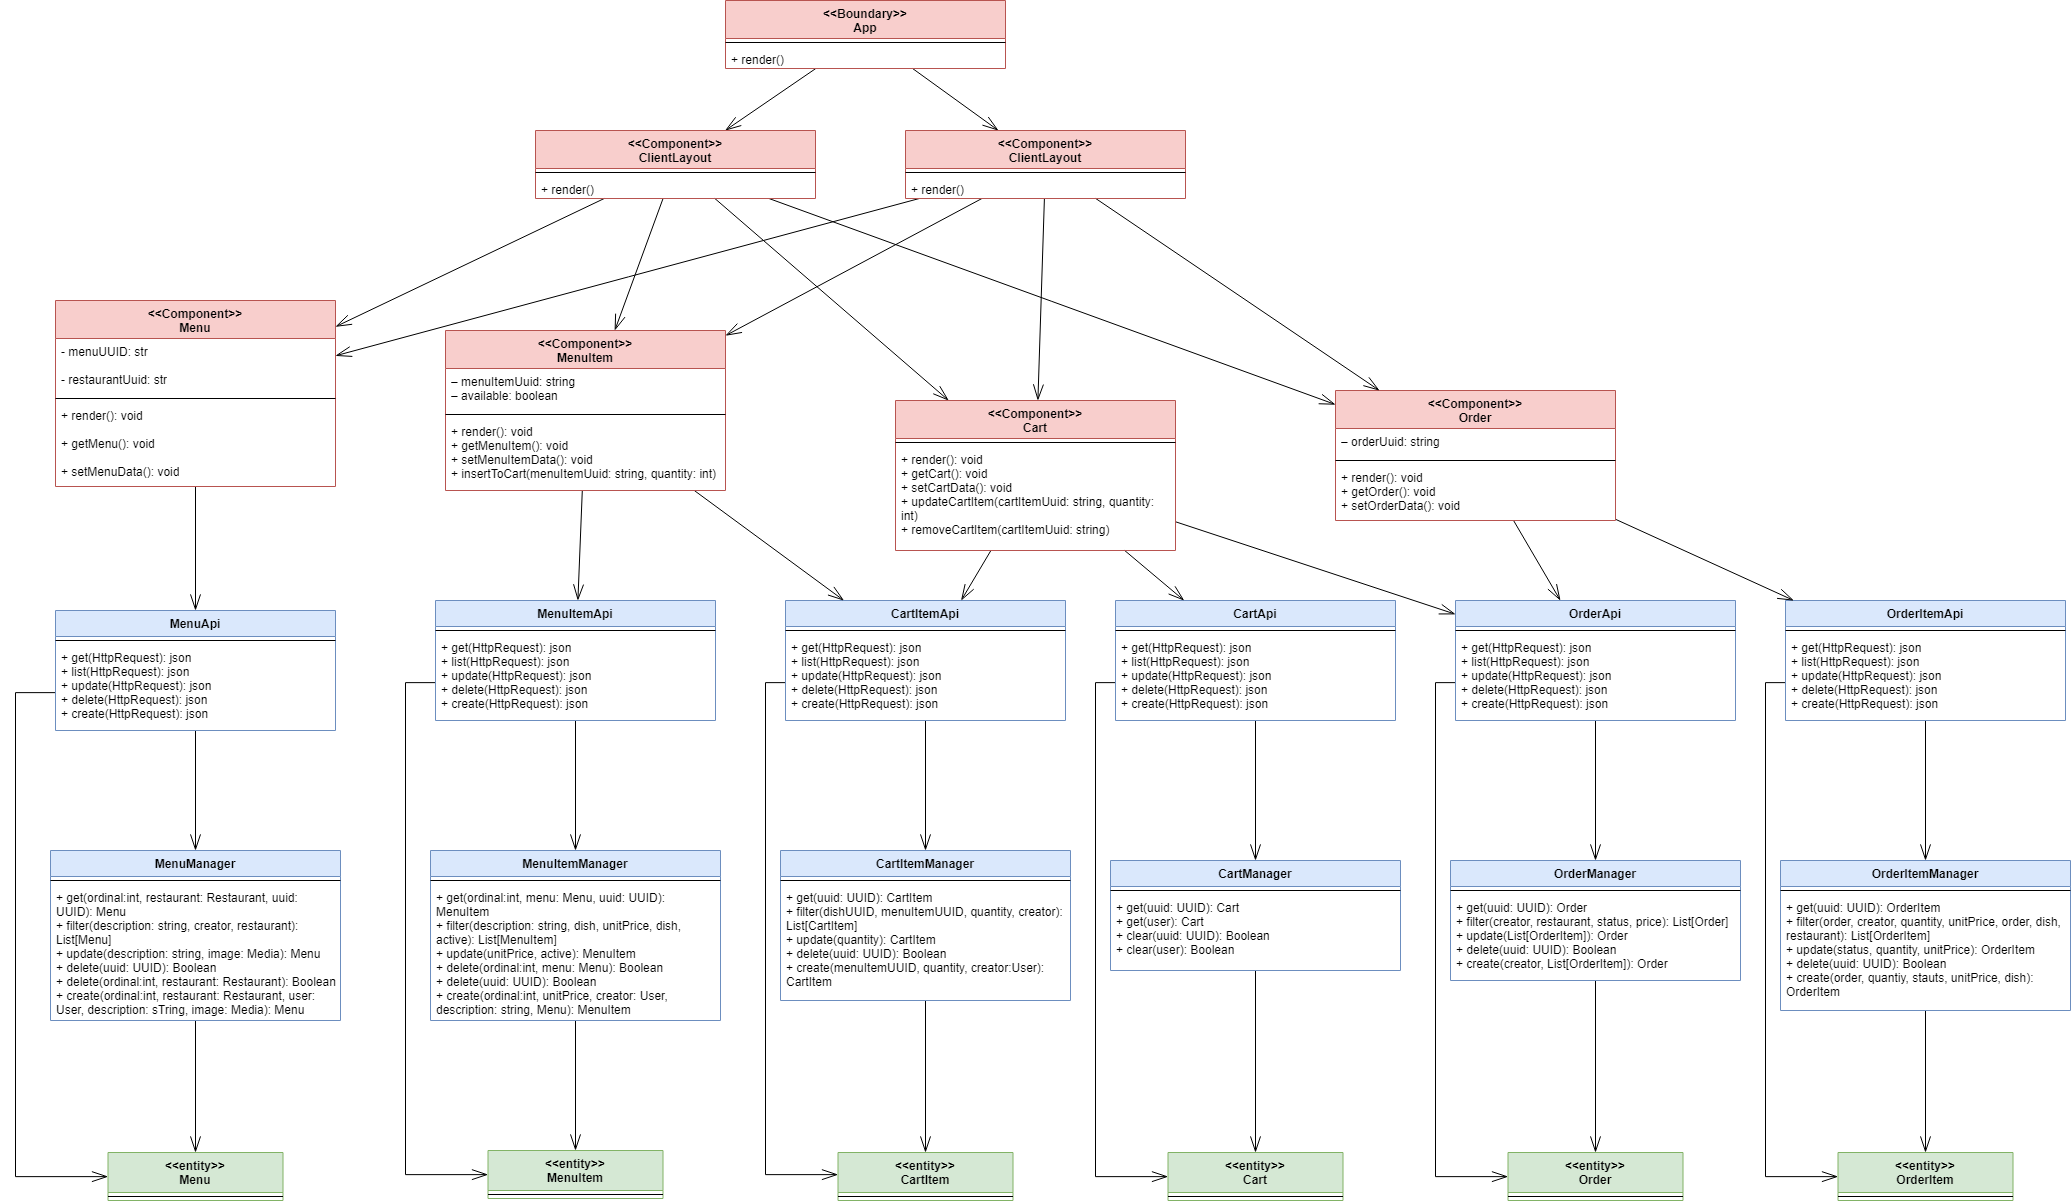
\includegraphics[scale=0.25,angle=90]{Images/ClassDiagram/order.png}
    \end{center}
    \hspace{0.3cm}
    \caption{entity class diagram}
\end{figure}
\newpage
\subsubsection{Mô tả diagram}
\subsubsubsection{class \textbf{ClientLayout}}
\begin{itemize}
    \item \textbf{Chức năng}: quản lý các component xuất hiện trong giao diện khách hàng.
    \item \textbf{Attributte} :
    \item \textbf{Methods}:
    \begin{itemize}
        \item render(): void
    \end{itemize}
\end{itemize}
\subsubsubsection{class \textbf{StaffLayout}}
\begin{itemize}
    \item \textbf{Chức năng}: quản lý các component xuất hiện trong giao diện nhân viên nhà hàng.
    \item \textbf{Attributte} :
    \item \textbf{Methods}:
    \begin{itemize}
        \item render(): void
    \end{itemize}
\end{itemize}
\subsubsubsection{class \textbf{Menu}}
\begin{itemize}
    \item \textbf{Chức năng}: Hiển thị menu của một nhà hàng.
    \item \textbf{Attributte} :
    \begin{itemize}
        \item restaurantUuid: string
    \end{itemize}
    \item \textbf{Methods}:
    \begin{itemize}
        \item[+] render(): void
        \item[+] getMenu(): void
        \item[+] setMenuData(): void
    \end{itemize}
\end{itemize}
\subsubsubsection{class \textbf{MenuItem}}
\begin{itemize}
    \item \textbf{Chức năng}: Hiển thị chi tiết một menu item của một nhà hàng.
    \item \textbf{Attributte} :
    \begin{itemize}
        \item menuItemUuid: string
        \item available: boolean
    \end{itemize}
    \item \textbf{Methods}:
    \begin{itemize}
        \item[+] render(): void
        \item[+] getMenuItem(): void
        \item[+] setMenuItemData(): void
        \item[+] insertToCart(menuItemUuid: string, quantity: int)
    \end{itemize}
\end{itemize}
\subsubsubsection{class \textbf{Cart}}
\begin{itemize}
    \item \textbf{Chức năng}: Hiển thị giỏ hàng của người dùng.
    \item \textbf{Attributte} :
    \item \textbf{Methods}:
    \begin{itemize}
        \item[+] render(): void
        \item[+] getCart(): void
        \item[+] setCartData(): void
        \item[+] updateCartItem(cartItemUuid: string, quantity: int)
        \item[+] removeCartItem(cartItemUuid: string)
    \end{itemize}
\end{itemize}
\subsubsubsection{class \textbf{Order}}
\begin{itemize}
    \item \textbf{Chức năng}: Hiển thị 1 đơn hàng của của 1 người dùng.
    \item \textbf{Attributte} :
    \begin{itemize}
        \item orderUuid: string
    \end{itemize}
    \item \textbf{Methods}:
    \begin{itemize}
        \item[+] render(): void
        \item[+] getOrder(): void
        \item[+] setOrderData(): void
    \end{itemize}
\end{itemize}
\subsubsubsection{class \textbf{MenuApi}}
\begin{itemize}
    \item \textbf{Chức năng}: Các api liên quan đến quản lý menu.
    \item \textbf{Attributte} :
    \item \textbf{Methods}:
    \begin{itemize}
        \item[+] get(HttpRequest): json
        \item[+] list(HttpRequest): json
        \item[+] update(HttpRequest): json
        \item[+] delete(HttpRequest): json
        \item[+] filter(HttpRequest): json
    \end{itemize}
\end{itemize}
\subsubsubsection{class \textbf{MenuItemApi}}
\begin{itemize}
    \item \textbf{Chức năng}: Các api liên quan đến quản lý MenuItem.
    \item \textbf{Attributte} :
    \item \textbf{Methods}:
    \begin{itemize}
        \item[+] get(HttpRequest): json
        \item[+] list(HttpRequest): json
        \item[+] update(HttpRequest): json
        \item[+] delete(HttpRequest): json
        \item[+] filter(HttpRequest): json
    \end{itemize}
\end{itemize}
\subsubsubsection{class \textbf{CartItemApi}}
\begin{itemize}
    \item \textbf{Chức năng}: Các api liên quan đến quản lý CartItem.
    \item \textbf{Attributte} :
    \item \textbf{Methods}:
    \begin{itemize}
        \item[+] get(HttpRequest): json
        \item[+] list(HttpRequest): json
        \item[+] update(HttpRequest): json
        \item[+] delete(HttpRequest): json
        \item[+] filter(HttpRequest): json
    \end{itemize}
\end{itemize}
\subsubsubsection{class \textbf{CartApi}}
\begin{itemize}
    \item \textbf{Chức năng}: Các api liên quan đến quản lý Cart.
    \item \textbf{Attributte} :
    \item \textbf{Methods}:
    \begin{itemize}
        \item[+] get(HttpRequest): json
        \item[+] list(HttpRequest): json
        \item[+] update(HttpRequest): json
        \item[+] delete(HttpRequest): json
        \item[+] create(HttpRequest): json
    \end{itemize}
\end{itemize}
\subsubsubsection{class \textbf{OrderItemApi}}
\begin{itemize}
    \item \textbf{Chức năng}: Các api liên quan đến quản lý OrderItem.
    \item \textbf{Attributte} :
    \item \textbf{Methods}:
    \begin{itemize}
        \item[+] get(HttpRequest): json
        \item[+] list(HttpRequest): json
        \item[+] update(HttpRequest): json
        \item[+] delete(HttpRequest): json
        \item[+] create(HttpRequest): json
    \end{itemize}
\end{itemize}
\subsubsubsection{class \textbf{OrderApi}}
\begin{itemize}
    \item \textbf{Chức năng}: Các api liên quan đến quản lý Order.
    \item \textbf{Attributte} :
    \item \textbf{Methods}:
    \begin{itemize}
        \item[+] get(HttpRequest): json
        \item[+] list(HttpRequest): json
        \item[+] update(HttpRequest): json
        \item[+] delete(HttpRequest): json
        \item[+] create(HttpRequest): json
    \end{itemize}
\end{itemize}
\subsubsubsection{class \textbf{MenuManager}}
\begin{itemize}
    \item \textbf{Chức năng}:  cung câp các method giúp query data từ table Menu và join các table khác nếu cần.
    \item \textbf{Attributte} :
    \item \textbf{Methods}:
    \begin{itemize}
        \item[+] get(ordinal:int, restaurant: Restaurant, uuid: UUID): Menu
        \item[+] filter(description: string, creator, restaurant): List[Menu]
        \item[+] update(description: string, image: Media): Menu
        \item[+] delete(uuid: UUID): Boolean
        \item[+] delete(ordinal:int, restaurant: Restaurant): Boolean
        \item[+] create(ordinal:int, restaurant: Restaurant, user: User, description: sTring, image: Media): Menu
    \end{itemize}
\end{itemize}
\subsubsubsection{class \textbf{MenuItemManager}}
\begin{itemize}
    \item \textbf{Chức năng}:  cung câp các method giúp query data từ table MenuItem và join các table khác nếu cần.
    \item \textbf{Attributte} :
    \item \textbf{Methods}:
    \begin{itemize}
        \item[+] get(ordinal:int, menu: Menu, uuid: UUID): MenuItem
        \item[+] filter(description: string, dish, unitPrice, dish, active): List[MenuItem]
        \item[+] update(unitPrice, active): MenuItem
        \item[+] delete(ordinal:int, menu: Menu): Boolean
        \item[+] delete(uuid: UUID): Boolean
        \item[+] create(ordinal:int, unitPrice, creator: User, description: string, Menu): MenuItem
    \end{itemize}
\end{itemize}
\subsubsubsection{class \textbf{CartItemManager}}
\begin{itemize}
    \item \textbf{Chức năng}:  cung câp các method giúp query data từ table CartItem và join các table khác nếu cần.
    \item \textbf{Attributte} :
    \item \textbf{Methods}:
    \begin{itemize}
        \item[+] get(uuid: UUID): CartItem
        \item[+] filter(dishUUID, menuItemUUID, quantity, creator): List[CartItem]
        \item[+] update(quantity): CartItem
        \item[+] delete(uuid: UUID): Boolean
        \item[+] create(menuItemUUID, quantity, creator:User): CartItem
    \end{itemize}
\end{itemize}
\subsubsubsection{class \textbf{CartManager}}
\begin{itemize}
    \item \textbf{Chức năng}:  cung câp các method giúp query data từ table Cart và join các table khác nếu cần.
    \item \textbf{Attributte} :
    \item \textbf{Methods}:
    \begin{itemize}
        \item[+] get(uuid: UUID): Cart
        \item[+] get(user): Cart
        \item[+] clear(uuid: UUID): Boolean
        \item[+] clear(user): Boolean
    \end{itemize}
\end{itemize}
\subsubsubsection{class \textbf{OrderManager}}
\begin{itemize}
    \item \textbf{Chức năng}:  cung câp các method giúp query data từ table Order và join các table khác nếu cần.
    \item \textbf{Attributte} :
    \item \textbf{Methods}:
    \begin{itemize}
        \item[+] get(uuid: UUID): Order
        \item[+] filter(creator, restaurant, status, price): List[Order]
        \item[+] update(List[OrderItem]): Order
        \item[+] delete(uuid: UUID): Boolean
        \item[+] create(creator, List[OrderItem]): Order
    \end{itemize}
\end{itemize}
\subsubsubsection{class \textbf{OrderItemManager}}
\begin{itemize}
    \item \textbf{Chức năng}:  cung câp các method giúp query data từ table OrderItem và join các table khác nếu cần.
    \item \textbf{Attributte} :
    \item \textbf{Methods}:
    \begin{itemize}
        \item[+] get(uuid: UUID): OrderItem
        \item[+] filter(order, creator, quantity, unitPrice, order, dish, restaurant): List[OrderItem]
        \item[+] update(status, quantity, unitPrice): OrderItem
        \item[+] delete(uuid: UUID): Boolean
        \item[+] create(order, quantiy, stauts, unitPrice, dish): OrderItem
    \end{itemize}
\end{itemize}
\newpage
\subsection{Xác thực tài khoản}

\begin{figure}[!h]
    \begin{center}
        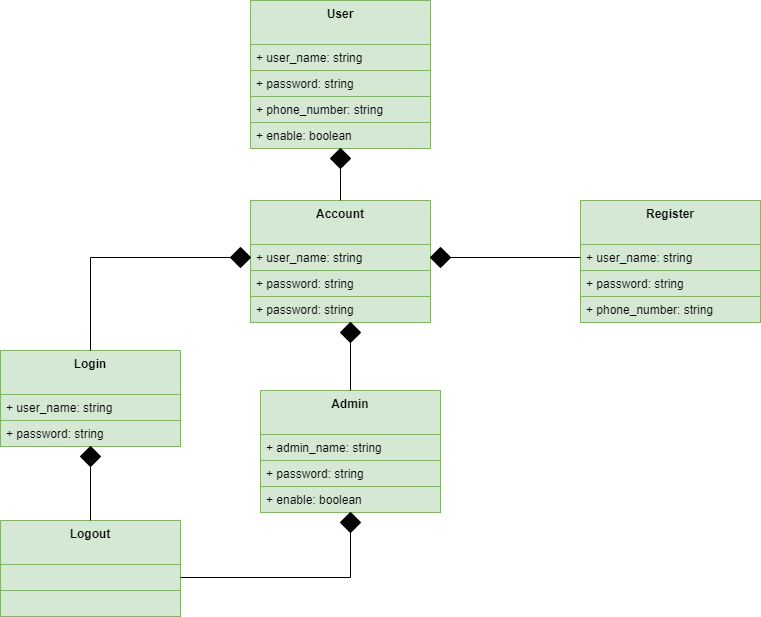
\includegraphics[scale=0.6]{Images/ClassDiagram/c_login.drawio.png}
    \end{center}
    \hspace{0.3cm}
    \caption{Xác thực tài khoản}
\end{figure}

\newpage
\subsection{Đặt bàn}

\begin{figure}[!h]
    \begin{center}
        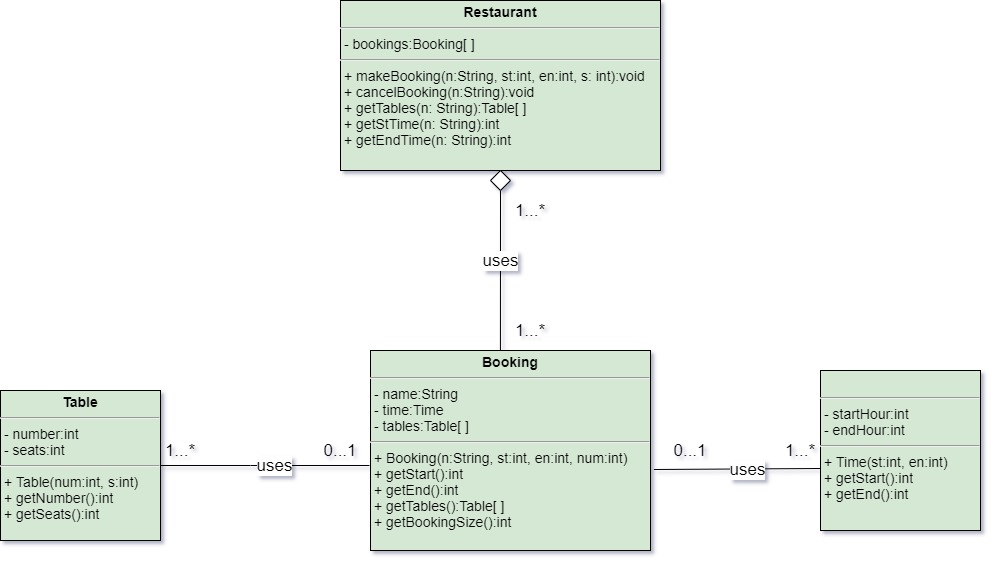
\includegraphics[scale=0.5]{Images/ClassDiagram/booking.jpg}
    \end{center}
    \hspace{0.3cm}
    \caption{Đặt bàn}
\end{figure}

\newpage
\subsection{Thanh Toán}

\begin{figure}[!h]
    \begin{center}
        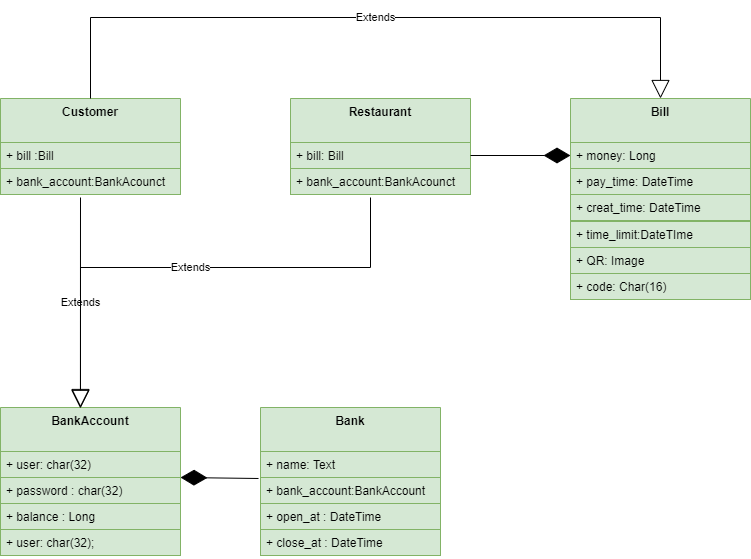
\includegraphics[scale=0.5]{Images/ClassDiagram/payment_class.png}
    \end{center}
    \hspace{0.3cm}
    \caption{Thanh toán}
\end{figure}

\newpage
\subsection{Quản lí nhà hàng}
\begin{figure}[!h]
    \begin{center}
        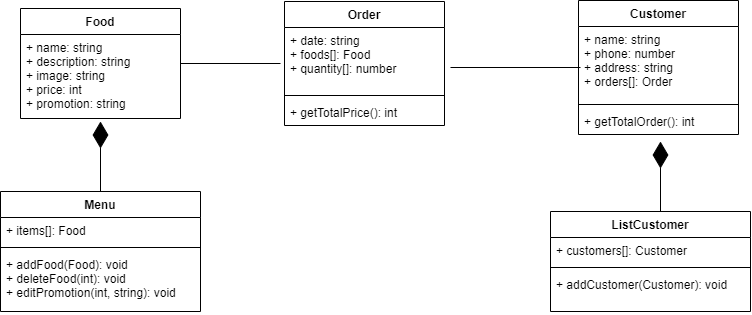
\includegraphics[scale=0.6]{Images/ClassDiagram/management.png}
    \end{center}
    \hspace{0.3cm}
    \caption{Class diagram quản lí nhà hàng}
\end{figure}
\newpage
\section{Thiết kế hệ thống}
- Hệ thống sử dụng mô hình MVC(Model - Controller - View) để thiết kế.
\begin{itemize}
    \item View: \\
    - Customer View: Chế độ mặc định khi truy cập vào trang chính của hệ thống, không yêu cầu mật khẩu, chỉ yêu cầu khách nhập số bàn đang ngồi của mình (có dán tại bàn). Dành cho khách hàng xem món, đặt món, thanh toán, gọi phục vụ và gửi phản hồi.\\
    - Waiter View: Chế độ dành cho phục vụ Cho phép phục vụ nhận thông báo khi có khách gọi hoặc có món cần giao và nhấn nút Nhận để xác nhận đã có phục vụ tiếp nhận yêu cầu.\\
    - Kitchen View: Chế độ dành cho bếp. Cho phép bếp tiếp nhận món được đặt, xác nhận hoặc từ chối, chuyển trạng thái của món để hệ thống thông báo cho khách và phục vụ.\\
    - Manager View: Chế độ dành cho quản lý. Cho phép quản lý chỉnh sửa thông tin, thêm hoặc xóa món và đọc phản hồi của người dùng.
    \item Model:\\
    - Lấy thông tin các món ăn có trong danh sách món ăn\\
    - Thông tin giỏ hàng khi khách hàng đặt món\\
    - Danh sách đơn hàng\\
    - Xử lí các giao dịch khi thanh toán\\
    - Nhận thông tin khách hàng phản hồi
    \item Controller:\\
    - Hiển thị các món ăn và số bàn còn trống cho khách hàng\\
    - Thêm hoặc xóa món ăn của khách hàng trong giỏ hàng\\
    - Xử lý những tương tác của nhân viên và khách hàng.\\
    - Xử lý việc thanh toán và phản hồi của khách hàng.\\
    - Xử lý việc cập nhật menu và thông tin các món ăn của nhân viên.\\
    - Lưu lại giao dịch và đánh giá của khách hàng, chỉnh sửa menu (thông tin các món ăn, giá tiền.....).
\end{itemize}
\begin{figure}[!h]
    \begin{center}
        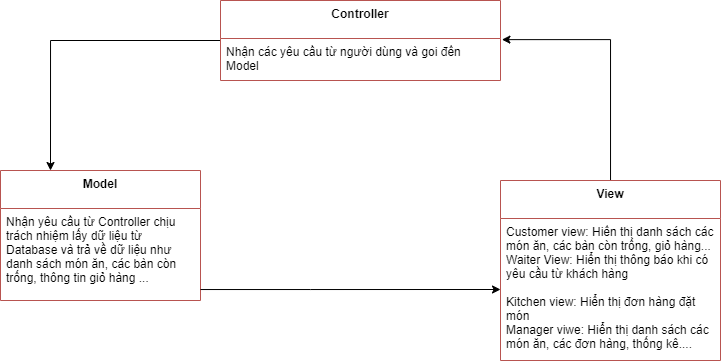
\includegraphics[scale=0.5]{Images/MVC.png}
    \end{center}
    \caption{Mô hình MVC}
\end{figure}
\newpage
\subsection{Deployment diagram}
\begin{figure}[!h]
    \begin{center}
        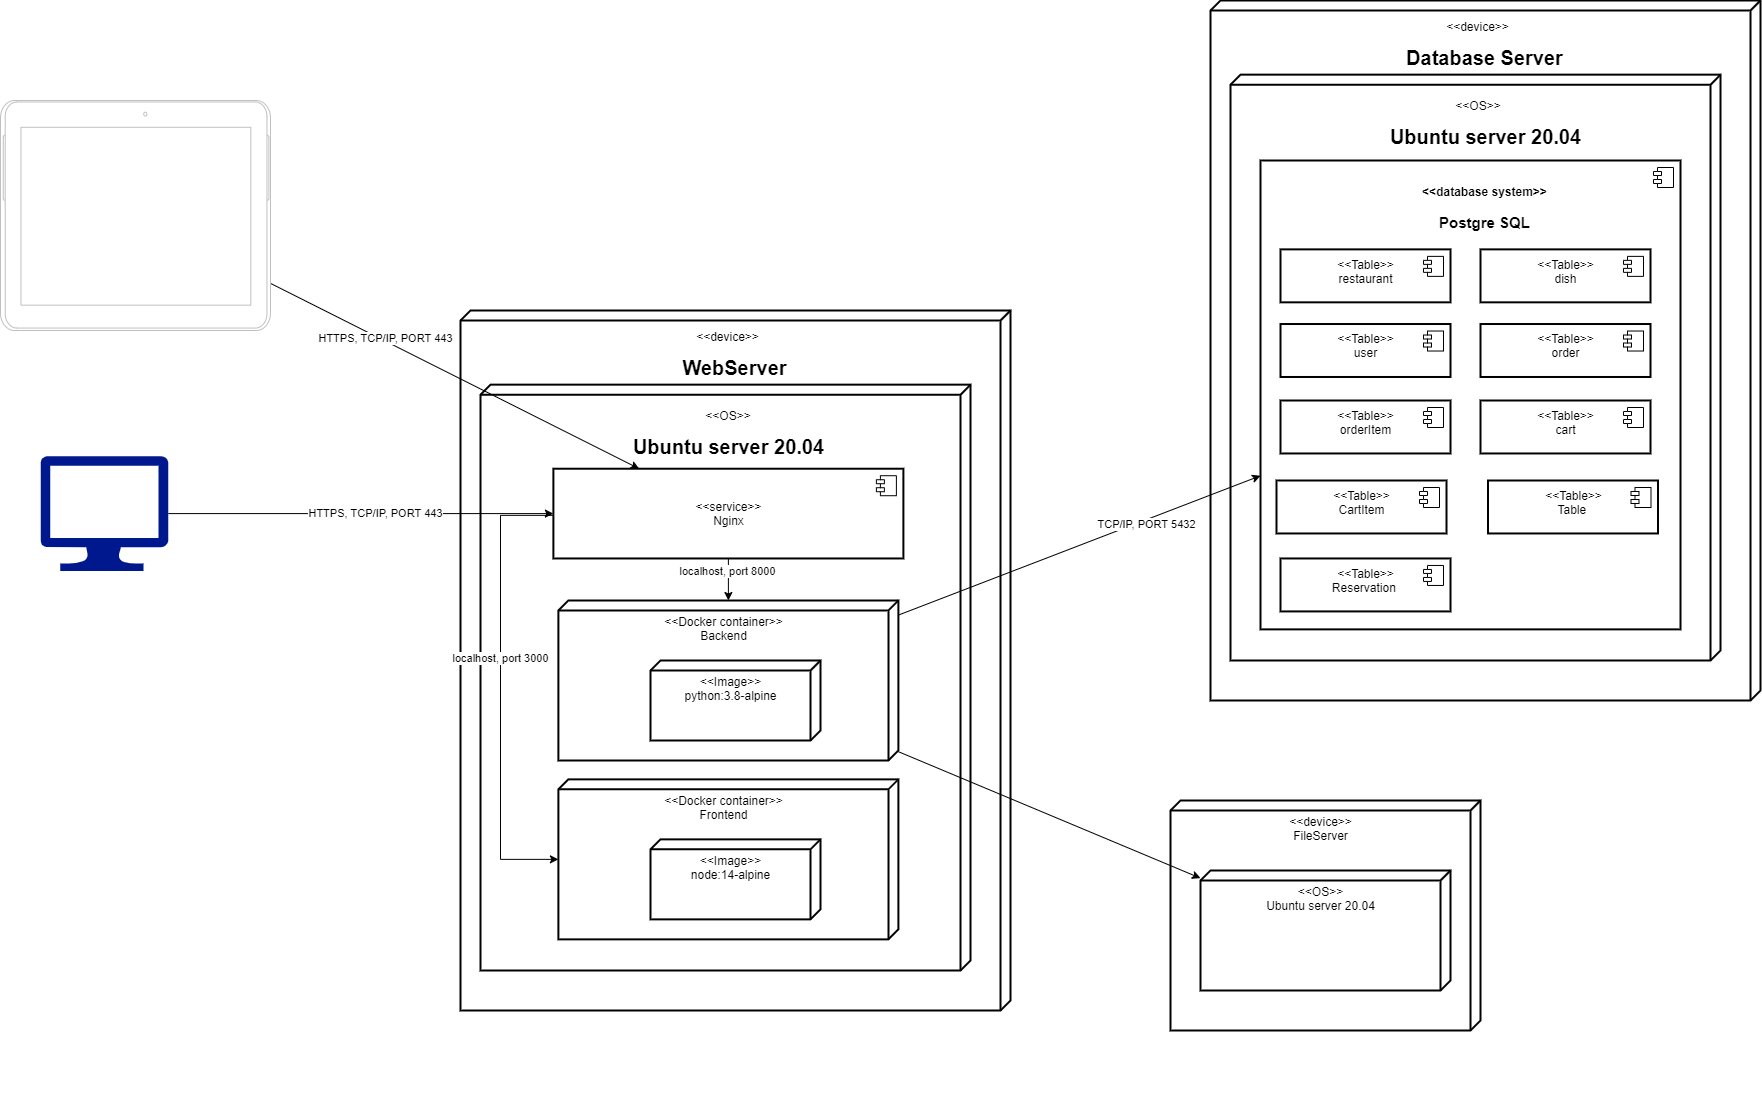
\includegraphics[scale=0.2]{Images/deploymet/SE_UML-deployment_diagram.png}
    \end{center}
    \caption{Deployment diagram}
\end{figure}

\newpage
\subsection{Component diagram}

\begin{figure}[!h]
    \begin{center}
        \includegraphics[scale=0.3]{Images/component.png}
    \end{center}
    \hspace{0.3cm}
    \caption{Component diagram}
\end{figure}

\section{Version Control System}

Nhóm sử dụng github làm version control system cho dự án.

Sé có 1 repo chính là se-2021. Repo sẽ gồm 3 sub-modules là se-backend, se-frontend và se-document.

Repositoies:
\begin{itemize}
    \item se-2021: \url{https://github.com/NQLong/se-2021.git}
    \item se-backend: \url{https://github.com/NQLong/se-backend.git}
    \item se-frontend: \url{https://github.com/NQLong/se-frontend.git}
    \item se-document: \url{https://github.com/NQLong/se-documents.git}
    
\end{itemize}
%%%%%%%%%%%%%%%%%%%%%%%%%%%%%%%%%
% \newpage
% \addcontentsline{toc}{section}{Tài liệu}
% \begin{thebibliography}{99999}
% % \bibitem[Dal]{Dal}{Dalgaard, P.} {\em Introductory Statistics with R.}  Springer 2008.

% % \bibitem[K-Z]{K-Z}{Kenett, R. S. and Zacks, S.}
% % {\em Modern Industrial Statistics: with applications in R, MINITAB and JMP,} 2nd ed.,  John Wiley and Sons, 2014.

% % \bibitem[Ker]{Ker}{Kerns, G. J.}
% % {\em Introduction to Probability and Statistics Using R,} 2nd ed., CRC 2015.
% \end{thebibliography}
\end{document}

